
\section{Analysis strategy}
\label{sec:analysis}

In this section we describe our analysis strategy.
%
First of all, we discuss the settings
for jet clustering  and the strategy for $b$-tagging.
%
Then we discuss the categorisation of events in different
topologies and how to prioritise among them.
%
We motivate our choice of analysis cuts by comparing signal and background
for representative kinematical distributions.
%
Finally, we describe the simulation of PU and validate
the PU subtraction strategy that we adopt.

\subsection{Jet reconstruction}

After the  parton shower, final state particles
are clustered using the
jet reconstruction algorithms
obtained from
{\tt FastJet}~\cite{Cacciari:2011ma,Cacciari:2005hq},
{\tt v3.1.0}.
%
We use different types of jet definitions:
\begin{itemize}
\item {\it Small-$R$ jets}.

  These are jets  reconstructed with the
  anti-$k_T$ clustering algorithm~\cite{Cacciari:2008gp} with $R=0.4$ radius.
  %
  These small-$R$ jets are required
  to have transverse momentum $p_T \ge 40$~GeV
  and pseudo-rapidity $|\eta|<2.5$, within the central 
  acceptance of ATLAS and CMS, the region
  where $b$-tagging is possible.

\item {\it Large-$R$ jets}.

  These jets are also constructed with the
  anti-$k_T$ clustering algorithm, now using a $R=1.2$ radius.
  %
  Large-$R$ jets are required to have
  $p_T \ge 200$~GeV and lie in a pseudo-rapidity region of
  $|\eta|<2.0$.
  %
  The more restrictive range  in pseudo-rapidity
  as compared to the small-$R$ jets
  is motivated by mimicking the  experimental requirements
  in ATLAS and CMS
  related to the track-jet based calibration~\cite{Aad:2014bia,ATLAS:2012kla}.

  In addition to the basic $p_T$ and $\eta$
  acceptance requirements, large-$R$ jets should also
  satisfy the  BDRS mass-drop tagger (MDT)~\cite{Butterworth:2008iy}
  conditions.
  %
  We use the {\tt FastJet} default
  parameters of  $\mu = 0.67$ and $y_{\textrm{cut}}= 0.09$.
  %
  Before applying the MDT, the large-$R$ jet
  constituents are reclustered with the Cambridge/Aachen (C/A)
  algorithm~\cite{Dokshitzer:1997in,Wobisch:1998wt}
  with $R=1.2$.

  
\item {\it Small-$R$ subjets}.

  These subjets are constructed by reclustering the constituents
  of a large-$R$ jet, again with  anti-$k_T$ algorithm,
  but this time with a smaller radius parameter, namely
  $R=0.3$~\cite{Aad:2015uka}.
 %
  These small-$R$ subjets will be the main input for
  $b$-tagging in the boosted category.
  %
  They are required to satisfy $p_T > 50$~GeV and $|\eta|<2.5$.
  %
\end{itemize}

In addition, we have
also explored the possible improvements
in the analysis from the use
of variable-$R$ jets~\cite{Krohn:2009zg}, finding
a similar performance as in the case of fixed-$R$ jets.
%
This is explained by the fact that
variable-$R$ jets are more suitable when
the degree of boost of the final state being reconstructed can span
a wide range~\cite{Cacciari:2008gd}, such as in heavy resonance
searches~\cite{Aad:2015fna},
where where the degree of boost of the final state
is {\it a priori} unknown.


For the   boosted and intermediate categories,
which involve the use of large-$R$ jets,
we will use jet substructure variables~\cite{Salam:2009jx,Aad:2013gja} to
improve the significance of the discrimination between signal and background
events in the MVA.
%
In particular we will consider the following jet
substructure variables:
\begin{itemize}
\item The $k_T$-splitting scale~\cite{Butterworth:2002tt,Butterworth:2008iy}.

  This variable is defined by reclustering the constituents of a jet with the
  $k_t$ algorithm~\cite{Ellis:1993tq},
  which usually clusters last the harder constituents, and then
  taking the $k_t$ distance measure between the two subjets at the final stage of the recombination
  procedure,
  \be
  \label{eq:ktsplitting}
\sqrt{d_{12}} \equiv {\rm min}\lp p_{T,1},p_{T,2}\rp \cdot \Delta R_{12} \, .
\ee
with $p_{T,1}$ and $p_{T,2}$ the transverse momenta of the two subjets merged
in the final step of the clustering, and $\Delta R_{12}$ the corresponding
angular separation.
  
\item The ratio of 2-to-1 subjettiness $\tau_{12}$~\cite{Thaler:2010tr,Thaler:2011gf}.

  The $N$-subjettiness variables $\tau_N$ are defined by clustering the constituents
  of a jet with the exclusive $k_t$ algorithm~\cite{Catani:1993hr}
  and requiring that $N$ subjets are found,
  \be
  \tau_N \equiv \frac{1}{d_0} \sum_k p_{T,k}\cdot {\rm min}\lp \delta R_{1k}, \ldots,
  \delta R_{Nk}\rp \, , \qquad d_0\equiv \sum_k p_{T,k}\cdot R \, ,
  \ee
  with $p_{T,k}$ is the $p_T$ of the constituent particle $k$ and $\delta R_{ik}$ the distance from
  subjet $i$ to constituent $k$.
  %
  In this work we use as input to the MVA the ratio of 2-subjettiness to 1-subjettiness
  \be
  \label{eq:tau21}
\tau_{21} \equiv \frac{\tau_2}{\tau_1} \, ,
  \ee
  which provides good discrimination power
  between QCD jets and jets arising from the decay of
  a heavy resonance.
  
\item The ratios of energy correlation functions (ECFs)  $C^{(\beta)}_2$~\cite{Larkoski:2013eya} and
  $D_2^{(\beta)}$~\cite{Larkoski:2014gra}.

  The ratio of energy correlation functions $C_2^{(\beta)}$ is defined as
  \be
  \label{eq:c2}
C_2^{(\beta)} \equiv \frac{ {\rm ECF}(3,\beta) {\rm ECF}(1,\beta)}{\lc {\rm ECF}(2,\beta)\rc ^2} \, ,
\ee
while $D_2^{(\beta)}$ is instead defined as a double ratio of ECFs, that is
\be
e_3^{(\beta)}\equiv \frac{ {\rm ECF}(3,\beta)}{\lc {\rm ECF}(1,\beta)\rc^3} \, , \quad
  e_2^{(\beta)}\equiv \frac{ {\rm ECF}(2,\beta)}{\lc {\rm ECF}(1,\beta)\rc^2} \, , \quad
  \label{eq:d2}
D_2^{(\beta)} \equiv \frac{ e_3^{(\beta)})}{\lp e_2^{(\beta)} \rp^3} \, .
\ee
The energy correlation functions ${\rm ECF}(N,\beta)$ are defined
  in~\cite{Larkoski:2013eya} with the motivation that $(N+1)$-point correlators
  are sensitive to $N$-prong substructure.
  %
  The free parameter $\beta$ is set to a value of $\beta=2$,
  as recommended by the authors of Refs.~\cite{Larkoski:2013eya,Larkoski:2014gra}.
\end{itemize}



\subsection{Tagging of $b$-jets}
\label{sec:btagging}

In this analysis we adopt
a $b$-tagging strategy along the lines
of current ATLAS performance~\cite{Aad:2013gja,Aad:2015ydr},
though differences with respect to
the corresponding CMS
settings~\cite{Khachatryan:2011wq,Chatrchyan:2012jua}
do not modify qualitatively our results.
%
For each type of jet definition used, a different
$b$-tagging strategy is adopted:

\begin{itemize}

\item {\it Small-$R$ jets}.

  %
  If a small-$R$ jet has at least one $b$-quark among their constituents,
  it will be tagged as a $b$-jet with probability $f_b$.
  %
  In order to be considered in the $b$-tagging algorithm,
  $b$-quarks inside the small-$R$ jet
  should satisfy $p_T \ge 15$ GeV~\cite{Aad:2015ydr}.
  %
  The probability of tagging a jet is not modified
  if more than one $b$-quark is found among the jet constituents.


  
  If no $b$-quarks are found among the constituents
  of this jet, it can be still be tagged as a $b$-jet with
  a mistag rate of $f_l$, unless a charm quark is present instead,
  and in this case the mistag rate is $f_c$.
  %
  Only jets that contain at least one (light or charm)
  constituent
  with $p_T \ge 15$ GeV can induce a fake $b$-tag.

  
  We attempt to $b$-tag only the four (two) hardest small-$R$ jets
  in the resolved (intermediate) category.
  %
  Trying to $b$-tag all the
  small-$R$ jets that satisfy the acceptance cuts worsens the
  overall performance
  due to combinatorics.

  \item {\it Large-$R$ jets}.

    Large-$R$ jets are $b$-tagged by
    ghost-associating anti-$k_T$ $R=0.3$ (AKT03)
    subjets to the original large-$R$
    jets~\cite{Cacciari:2007fd,Aad:2013gja,
      ATLAS-CONF-2014-004,Aad:2015uka}.
    %
    A large-$R$ jet will considered $b$-tagged if both
    the leading and subleading AK03 subjets, where the ordering
    is done in the subjet $p_T$, are both individually $b$-tagged,
    with the same criteria as the small-$R$ jets.
    %
     Therefore, a large-$R$ jet where the two leading
    subjets have at least one $b$-quark will be tagged
    with probability $f_b^2$.
    
    As in the case
    of small-$R$ jets, we only attempt to $b$-tag the two leading subjets,
    else one finds a degradation of the
    signal significance due to combinatorics.
    %
    The treatment of the $b$-jet mis-identification
    from light and charm jets
    is the same as for the small-$R$ jets.
  
\end{itemize}

Concerning the values of the $b$-tag probability, $f_b$, and
the $b$-mistag probability of light and charm jets, $f_l$ and  $f_c$
respectively,
we used the values $f_b=0.8$, $f_l=0.01$
and  $f_c=0.1$.





\subsection{Event categorisation}
\label{sec:categorisation}

The basic idea of the present analysis is similar to the
scale-invariant resonance tagging introduced
in Ref.~\cite{Gouzevitch:2013qca}.
%
Rather than restricting to a specific event topology,
we aim to consistently combine the information from
the three possible topologies: boosted, intermediate and
resolved.
%
The optimal cuts for each category will be determined
separately, and then
a exclusive categorisation is defined starting from the category
with the highest signal significance.
%
An advantage of our approach
the robustness under variations of
the underlying production model of Higgs pairs is modified,
for instance in the case of
BSM dynamics, which can substantially increase
the degree of boost of the final state.


These three categories are defined as follows:
\begin{itemize}
\item {\it Boosted category}.

  An event which
  contains at least two large-$R$ jets, with the two leading jets
 being $b$-tagged.
 %
 Each of these two large-$R$, $b$-tagged, jets are 
 thus candidates
 to contain the decay products of a Higgs boson.

\item {\it Intermediate category}.

  An event with exactly one large-$R$, $b$-tagged, jet, which
  is assigned to be the leading Higgs candidate.
  %
  In addition, we require at least two small-$R$, $b$-tagged, jets,
  which must be separated with respect to the large-$R$ jet
  by an angular distance of $\Delta R\ge 1.2$.
  %
    
  The subleading Higgs boson candidate is reconstructed
  by selecting the two $b$-tagged small-$R$ jets that minimize the difference
  between the invariant mass of the large-$R$ jet
  with that of the dijet obtained
  from the sum of the two small-$R$ jets.
  
\item {\it Resolved category}.

  
 An event with at least
  four $b$-tagged small-$R$ jets.
  %
  The two Higgs candidates are reconstructed out of the
  leading four small-$R$ jets in the event
  by considering all possibilities of forming two pairs of jets
  and then choosing the configuration that minimizes the relative difference of
  dijet masses.
  %
  
\end{itemize}


Once a Higgs boson candidate has been identified,
its invariant mass is required to lie within a fixed window
around the nominal Higgs boson mass of $m_h= 125$
GeV.
%
In particular we require the condition
\be
\label{higgsmasswindow}
|m_{h,j} - 125| < 40~{\rm GeV} \, ,\, j=1,2 \, ,
\ee
where $m_{h,j}$ is the invariant mass of each of the two reconstructed  Higgs candidates.
%
This cut is substantially looser as the corresponding
cut used in the typical ATLAS and CMS $h\to b\bar{b}$
analyses~\cite{Aad:2012gxa,Chatrchyan:2013zna}: the motivation
for this choice is that the MVA will take care of the optimisation of this,
as well as of other cuts that are not explicitly performed.
%
Only events where the two Higgs candidates satisfy
Eq.~(\ref{higgsmasswindow}) are classified as signal events.
%

These three categories are not exclusive:
a given event can be assigned to more than one category, for
example, satisfying the requirements of both the intermediate
and resolved
categories at the same time.
%
The exception is the boosted and intermediate categories, which have
orthogonal jet selection requirements.
%
The separate optimisation of the three categories needs to be performed in
a inclusive analysis, and then we introduce a
 priorisation starting with the category of highest signal significance.


 This has been achieved as follows.
 %
First of all we perform an inclusive analysis, and optimise the
signal significance
$S/\sqrt{B}$ in each of the three categories separately, including
the MVA.
%
We find that the category with higher significance turns out to be
the boosted one,
followed by the intermediate and the resolved ones, the latter two
with similar significance.
%
Therefore, for the final analysis, we turn to an exclusive approach:
if an event satisfies the boosted requirements, it is assigned to
this category, else we check if it suits the intermediate
requirements, and failing also this, the event is attempted to
be classified in the
resolved category.
%
The resulting exclusive event samples are then separately processed
through the MVA, allowing a consistent combination
of the significance of the three event categories.

\subsection{Motivation for basic kinematic cuts}

We now motivate the values of
kinematic cuts applied to the different categories, 
comparing representative kinematic distributions between
signal and background events.
%
First to all, we present results without PU, and in the next
subsection we discuss the impact of PU
on the description of the various kinematic
distributions.
%
In the following, all
distributions will be normalized to their total integral.

%
To begin with,
in Fig.~\ref{fig:cutplots1} we show
the $p_T$ distributions
of the
  leading and subleading large-$R$ jets in the boosted category, comparing
  the shapes of the distribution in signal and background events.
  %
  We see that the background distribution
  falls off rather steeply than the signal at large $p_T$
  for the two Higgs candidates.
  %
  On the other hand, the cut in $p_T$ cannot be too strong to avoid
  a substantial degradation of signal selection efficiency,
  specially taking into account the subleading large-$R$ jet.
  %
  This comparison justifies the cut of $p_T \ge 200$ GeV
  for the large-$R$ jets that we impose in the boosted category.
  

%%%%%%%%%%%%%%%%%%%%%%%%%%%%%%%%%%%%
\begin{figure}[t]
\begin{center}
 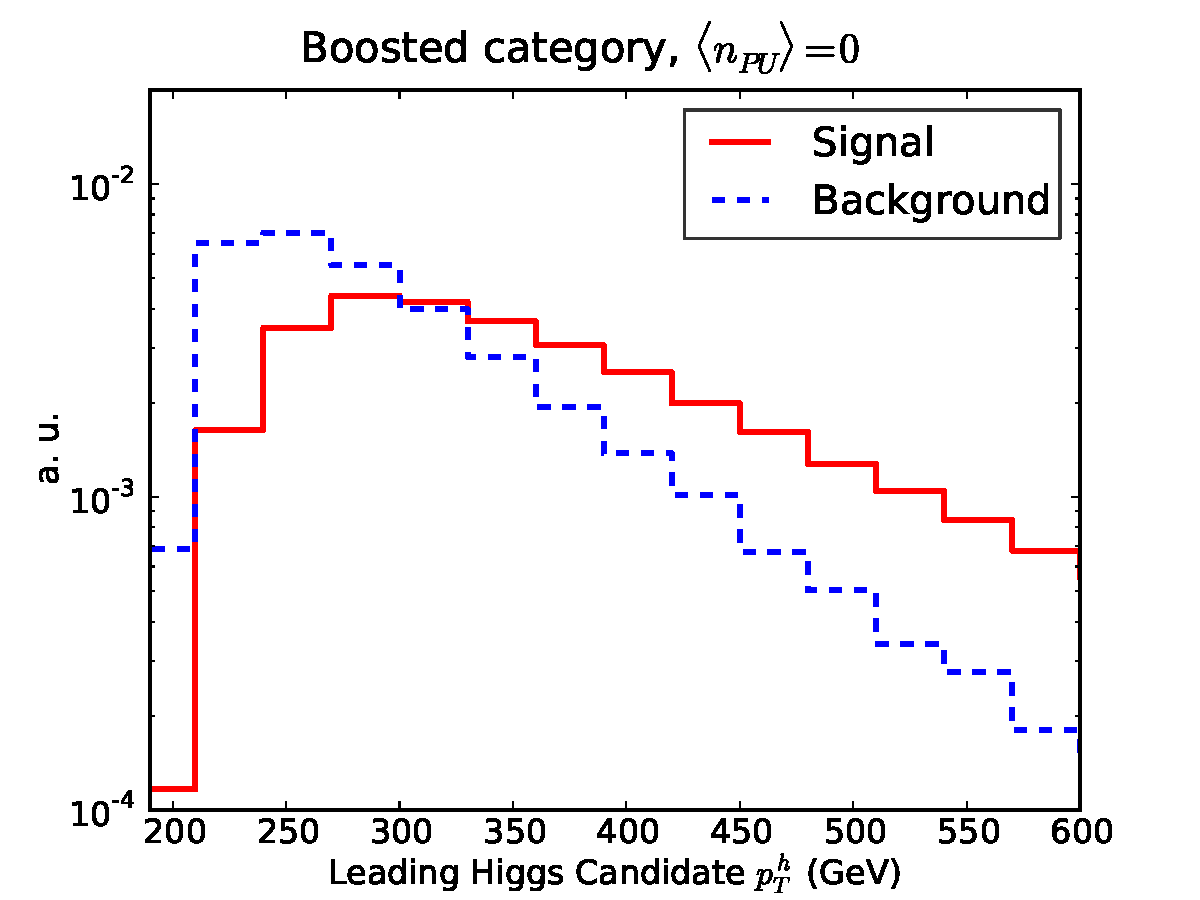
\includegraphics[width=0.48\textwidth]{plots/pt_H0_bst_C1d_noPU.pdf}
 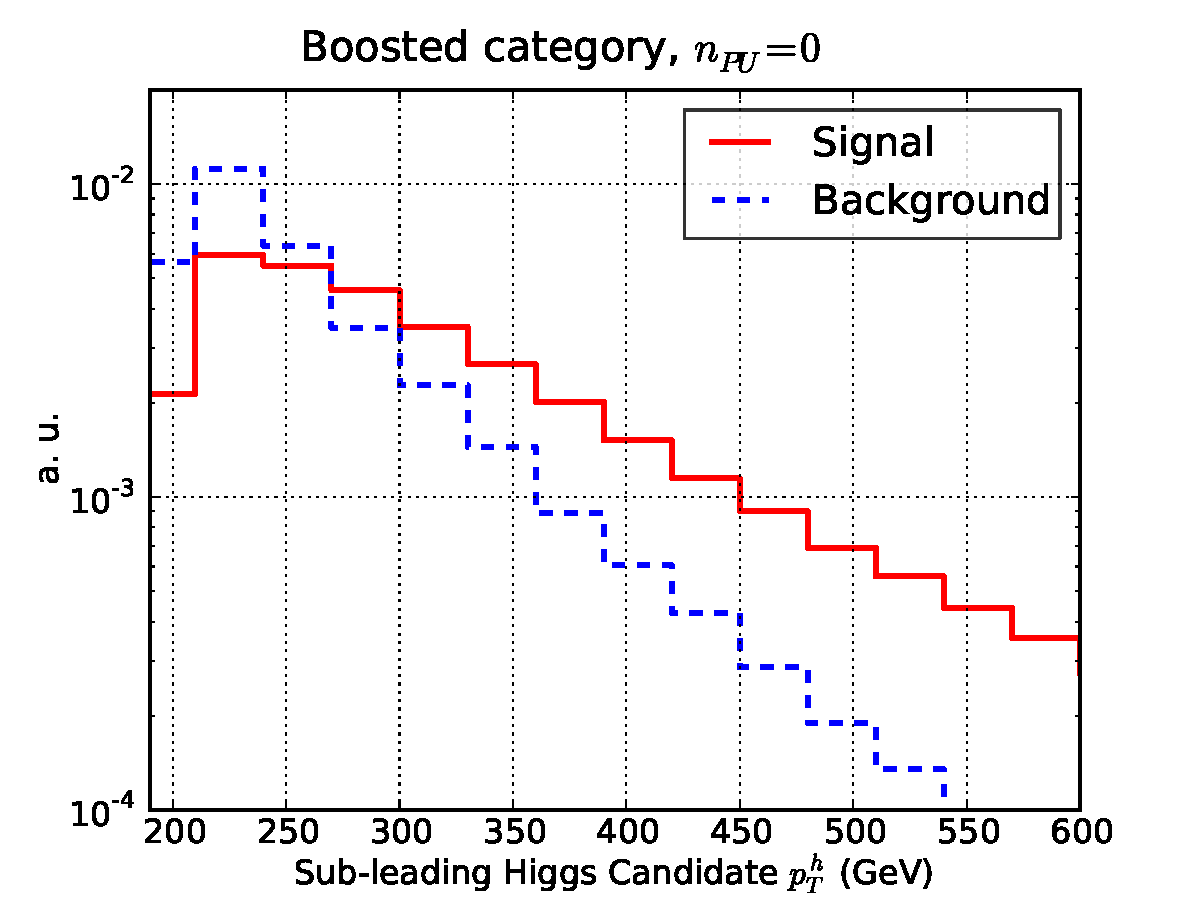
\includegraphics[width=0.48\textwidth]{plots/pt_H1_bst_C1d_noPU.pdf}
\caption{\small  Comparison of the $p_T$ distributions of the
  leading (left plot) and
  subleading (right plot) large-$R$ jets in the boosted category,
  in in signal and background events.
  %
  Distributions have been normalized to unity.
}
\label{fig:cutplots1}
\end{center}
\end{figure}
%%%%%%%%%%%%%%%%%%%%%%%


Another selection requirement for the boosted category is that the two
leading AKT03 subjets of the large-$R$ jet must be relatively hard,
in particular they should satisfy $p_T \ge $ 50 GeV.
%
To motivate this cut, in Fig.~\ref{fig:cutplots22}
we show the distribution in $p_T$ of the leading
and subleading AKT03 subjets in the subleading large-$R$ jet in events
corresponding to the boosted category.
%
It is clear from the comparison that the subjet $p_T$ spectrum is
relatively harder in the signal with respect to the background.
%
On the other hand, considering the subleading AKT03 subjet,
this cut in its  $p_T$
cannot be too harsh, to maintain a high signal selection
efficiency.
%
Therefore,
as for the previous distribution, also here 
a compromise between suppressing backgrounds but keeping a large fraction of
signal events is crucial.


%%%%%%%%%%%%%%%%%%%%%%%%%%%%%%%%%%%%
\begin{figure}[t]
\begin{center}
 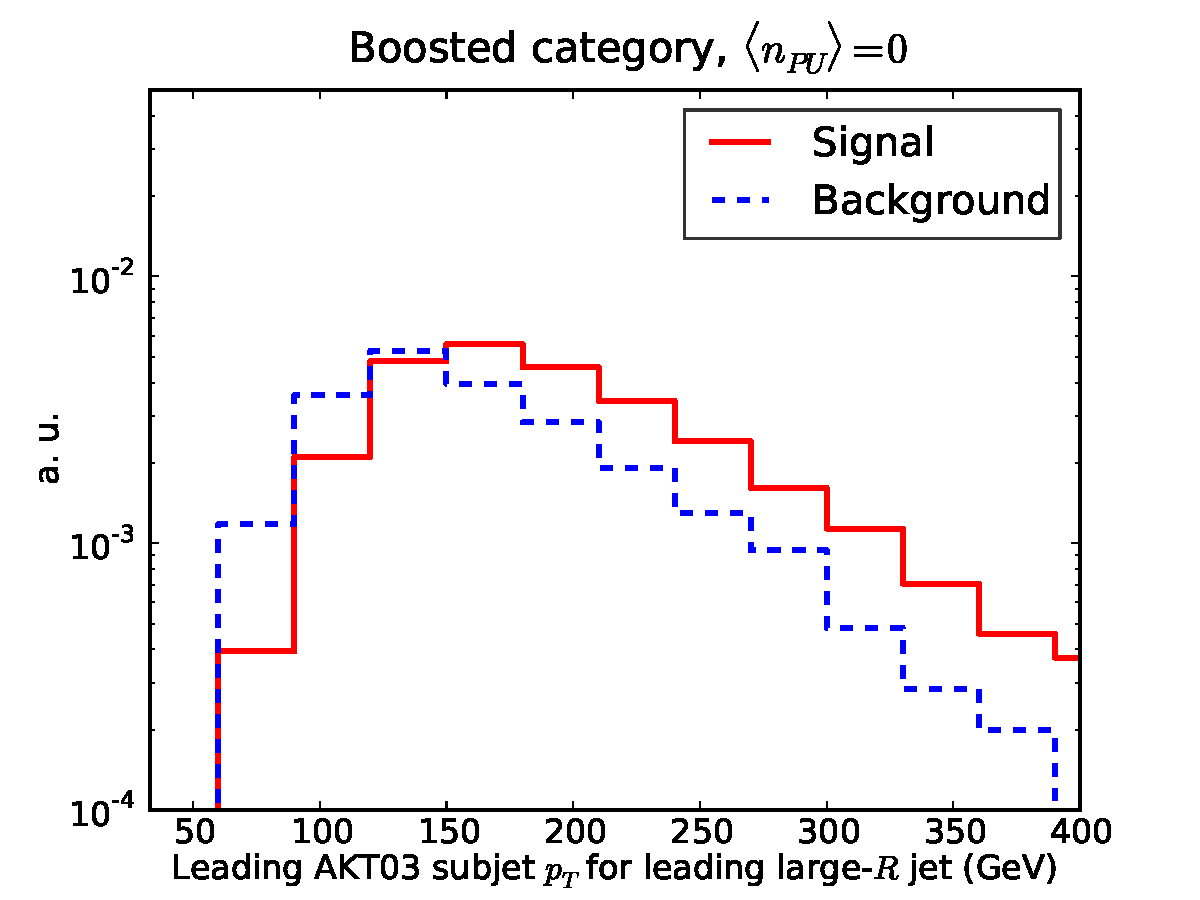
\includegraphics[width=0.48\textwidth]{plots/pt_leadSJ_fj2_noPU.pdf}
 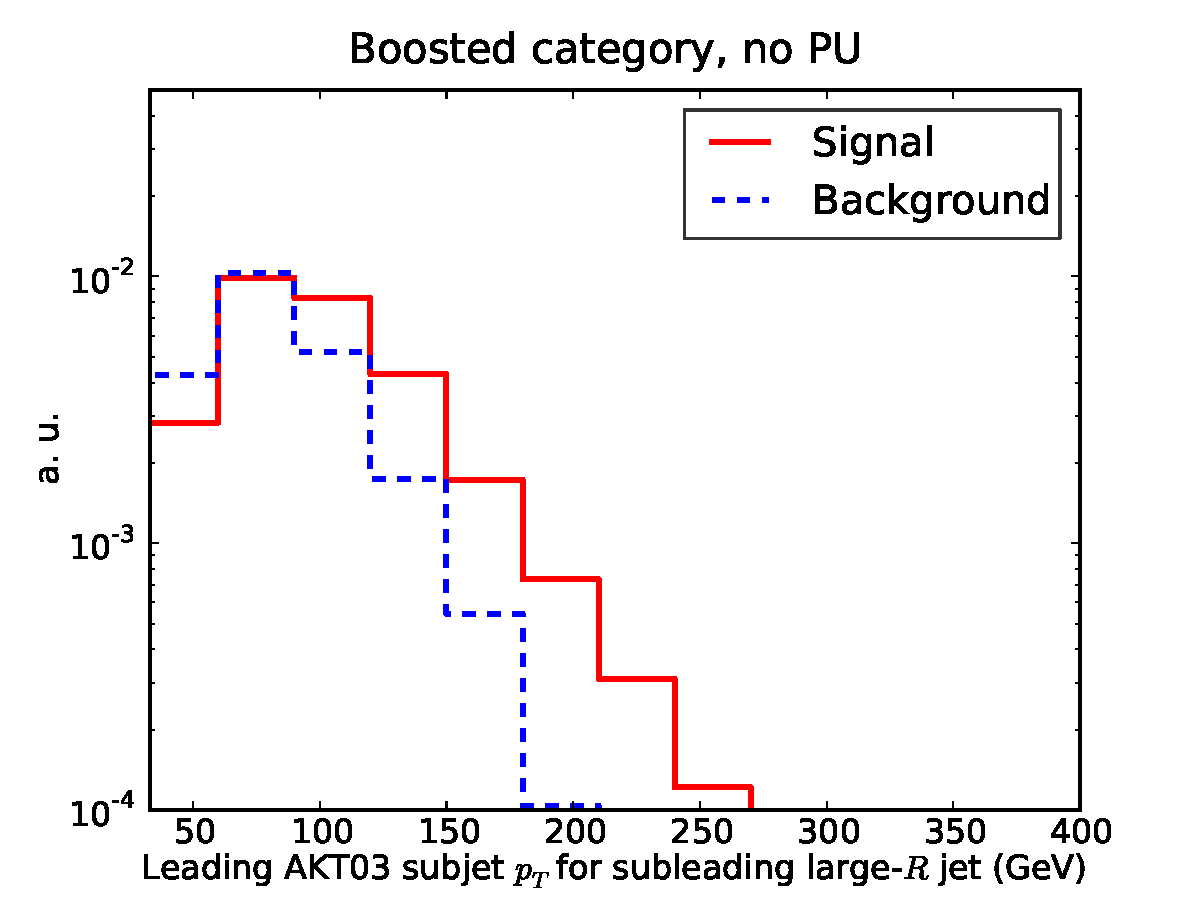
\includegraphics[width=0.48\textwidth]{plots/pt_subleadSJ_fj2_noPU.pdf}
 \caption{\small  Same as Fig.~\ref{fig:cutplots1} for the two leading AKT03
   subjets in the subleading Higgs candidate large-$R$ jet.
}
\label{fig:cutplots22}
\end{center}
\end{figure}
%%%%%%%%%%%%%%%%%%%%%%%


Turning to the resolved category, an important aspect to account
in the corresponding selection
cuts is the fact that the $p_T$ distribution
of the four leading small-$R$ jets of the event can be relatively soft,
specially for the subleading jets.
%
As noted in~\cite{deLima:2014dta}, this is a consequence of the fact
that in general the boost from the Higgs decays is moderate.
%
These considerations lead to the requirement that the $p_T$ cut
for the small-$R$ jets cannot be too strong.
%
In Fig.~\ref{fig:cutplots23}
we show the distribution in $p_T$ of the four leading
small-$R$ jets in signal and background events: we observe that both
distributions are peaked at $p_T \le 50$ GeV, with the signal distribution
eventually becoming dominant at large $p_T$.
%
The feasibility to being able to trigger on four small-$R$ jets with a relatively
soft $p_T$ distribution is one of the experimental challenges of
exploiting the resolved category in this final state,
and hence the requirement that $p_T \ge 40$ GeV for
the small-$R$ jets.
%
In  Fig.~\ref{fig:cutplots23} we also show the
rapidity distribution of the the small-$R$
jets in the resolved category: as well know, the production
is mostly central (more in the case
of signal events, since backgrounds are dominated by
QCD $t$-channel exchange) and thus the standard rapidity cuts
are relatively harmless.



%%%%%%%%%%%%%%%%%%%%%%%%%%%%%%%%%%%%
\begin{figure}[t]
\begin{center}
 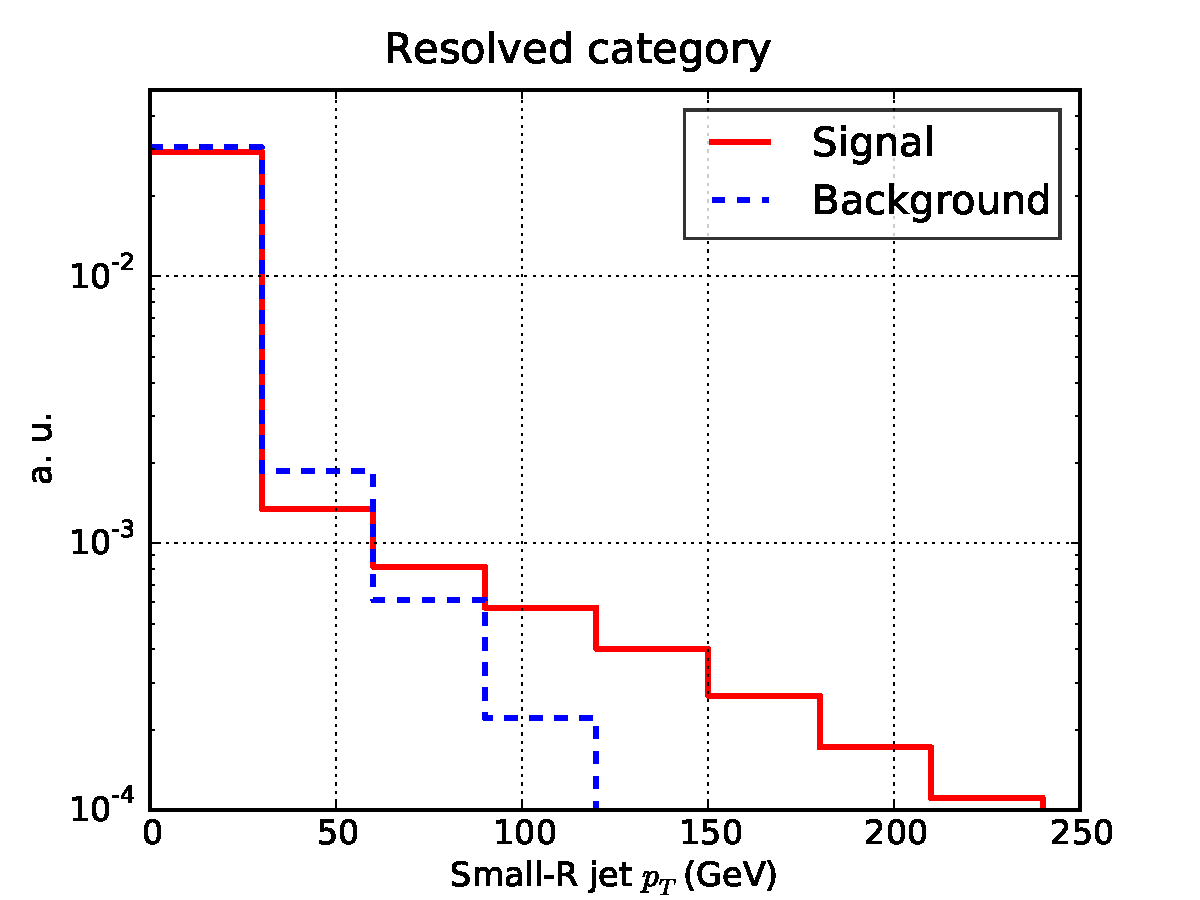
\includegraphics[width=0.48\textwidth]{plots/pt_smallRjets_res_noPU.pdf}
 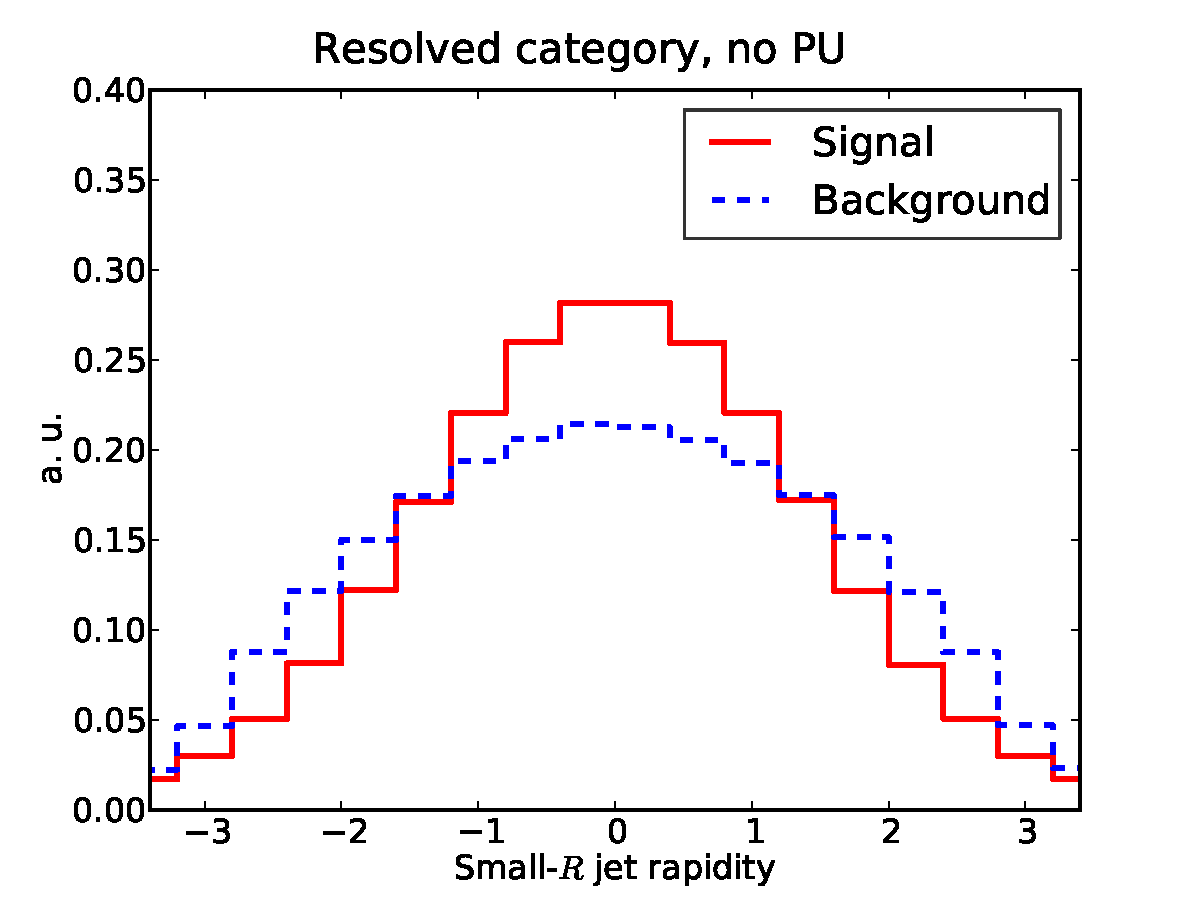
\includegraphics[width=0.48\textwidth]{plots/eta_smallRjets_res_noPU.pdf}
 \caption{\small Same as Fig.~\ref{fig:cutplots1}, now for the
   $p_T$ and rapidity distributions of the small-$R$
   jets corresponding to the resolved selection.
}
\label{fig:cutplots23}
\end{center}
\end{figure}
%%%%%%%%%%%%%%%%%%%%%%%

One of the selection cuts with highest discrimination power is the requirement
that the invariant mass of the Higgs candidate (di)jets must lie within a window
around the nominal Higgs value, Eq.~(\ref{higgsmasswindow}).
%
In Fig.~\ref{fig:mHHinv} we show the invariant mass
of the leading reconstructed Higgs candidates, before the Higgs mass window
cut 
  is applied, for the resolved and boosted categories.
%
While the signal distribution is of course peaked at the
nominal Higgs mass, the background distributions
show no particular
structure.
%
The
width of the Higgs mass peak is driven both from QCD effects,
such as initial-state radiation (ISR)
and out-of-cone radiation, as well
as from the four-momenta smearing applied to final state particles.
%

%%%%%%%%%%%%%%%%%%%%%%%%%%%%
\begin{figure}[t]
\begin{center}
  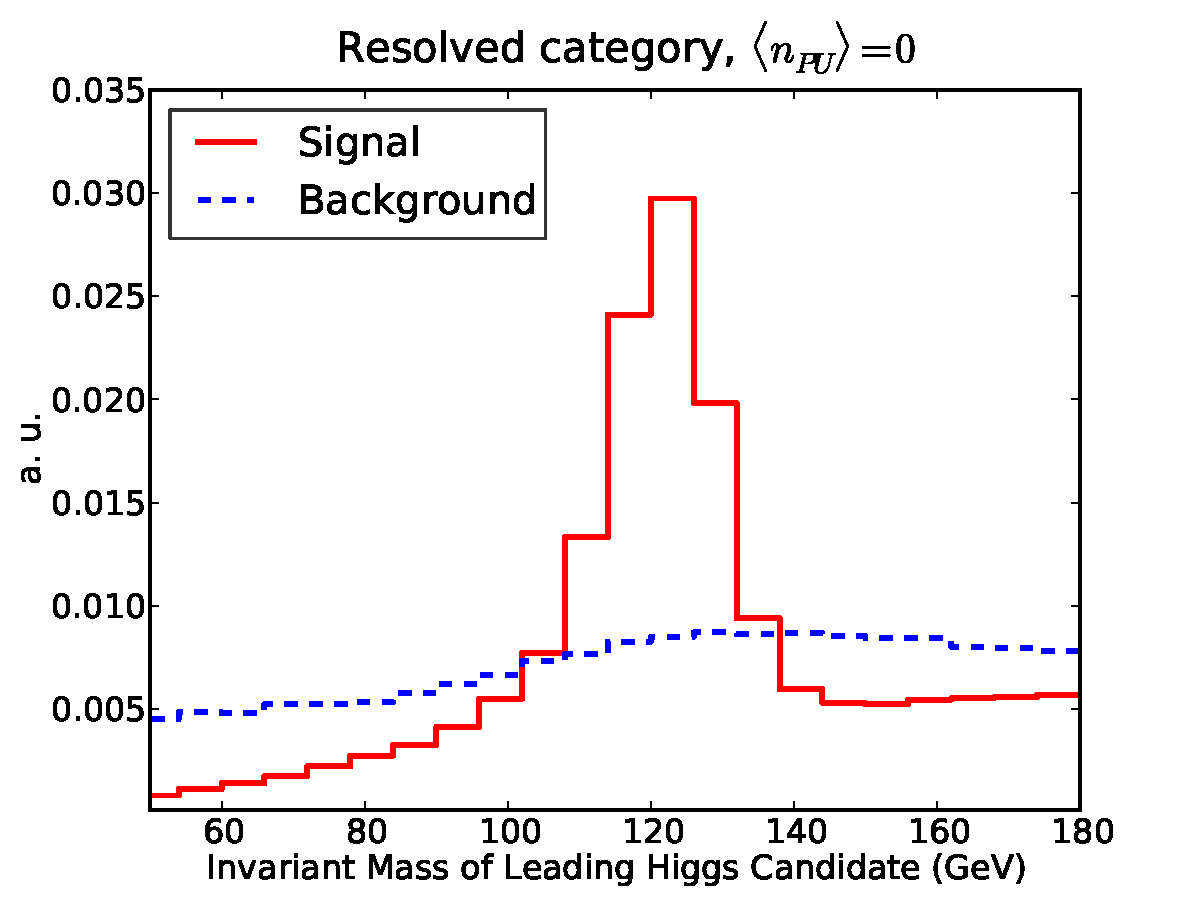
\includegraphics[width=0.48\textwidth]{plots/m_H0_res_C1d_noPU.pdf}
  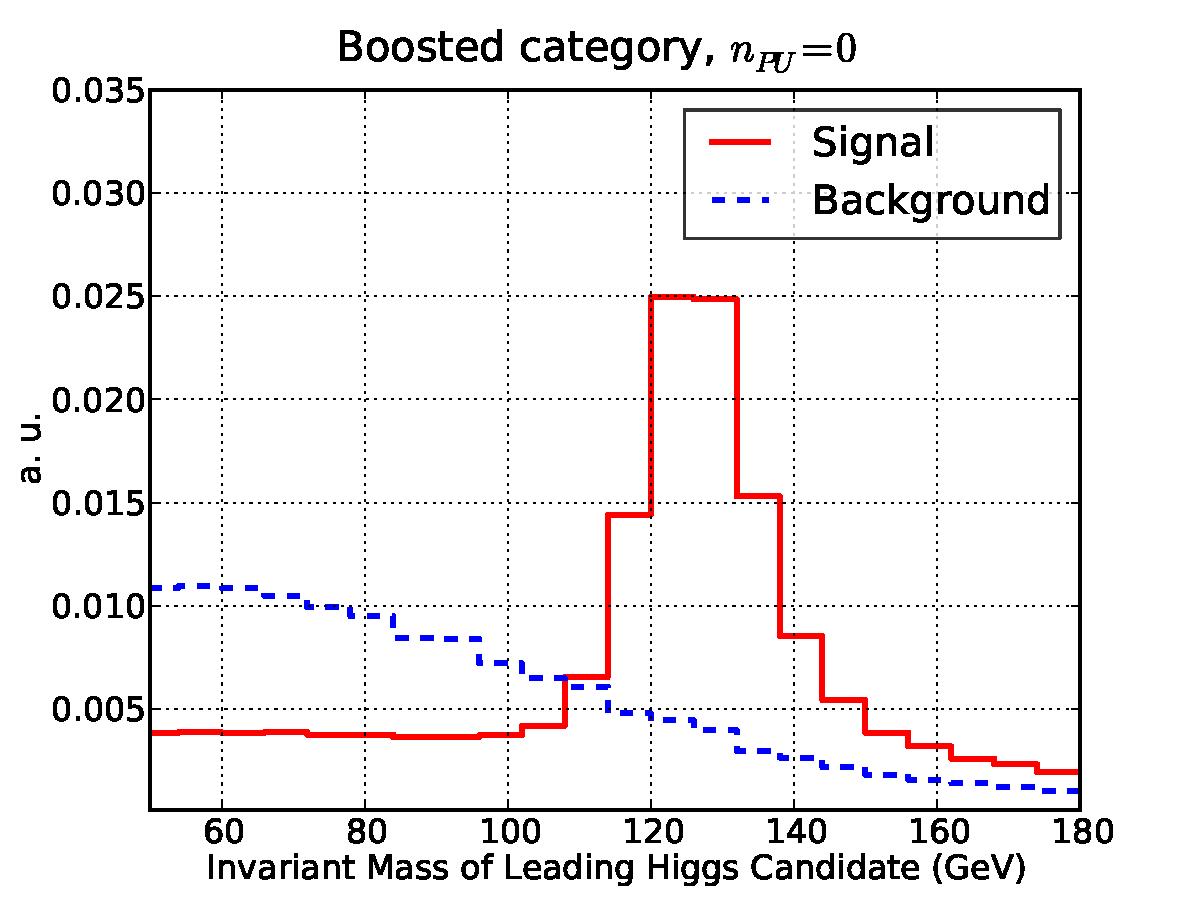
\includegraphics[width=0.48\textwidth]{plots/m_H0_bst_C1d_noPU.pdf}
  \caption{\small Same as   Fig.~\ref{fig:cutplots1} for the invariant
    mass distribution of the leading Higgs candidates in the resolved
    (left plot) and boosted (right plot) selections.
}
\label{fig:mHHinv}
\end{center}
\end{figure}
%%%%%%%%%%%%%%%%%%%%%%%


Another important kinematic distribution of this process is the invariant mass
of the di-Higgs system.
%
This is a direct measure of the boost of the system,
which in  BSM scenarios can be substantially
enhanced, for instance due to
of specific $d=6$ EFT operators~\cite{Azatov:2015oxa}.
%
One important advantage of the $b\bar{b}b\bar{b}$ final state for
di-Higgs production is that it significantly increases the reach
in $m_{hh}$ as compared to other channels with smaller branching
ratios,
such as $2b2\gamma$ or $2b2\tau$.
%
In Fig.~\ref{fig:mhh} we show the invariant mass distribution of the
reconstructed Higgs pairs,
comparing the resolved and the boosted categories.

%%%%%%%%%%%%%%%%%%%%%%%%%%%%%%%%%%%%%%%%%%%%%%%
\begin{figure}[t]
\begin{center}
  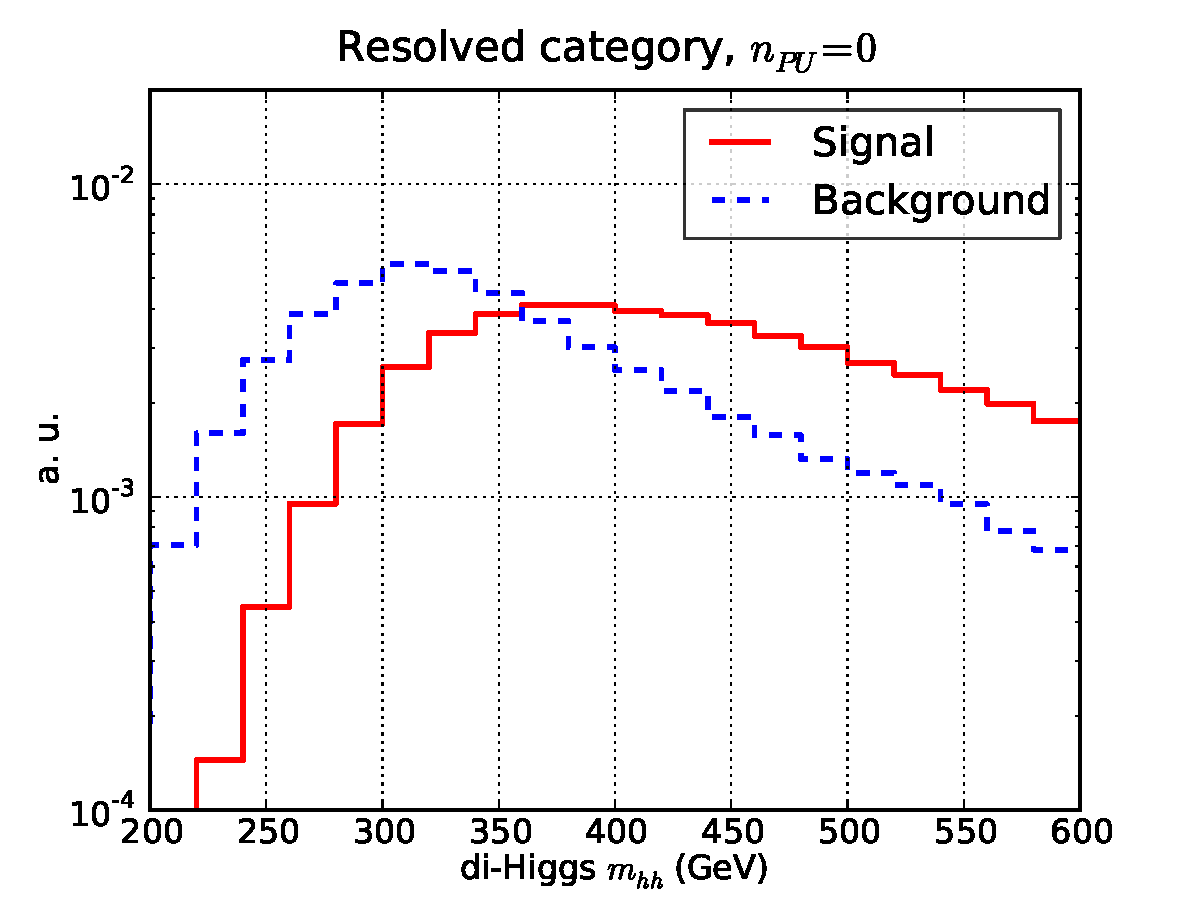
\includegraphics[width=0.48\textwidth]{plots/m_HH_C2_res_noPU.pdf}
  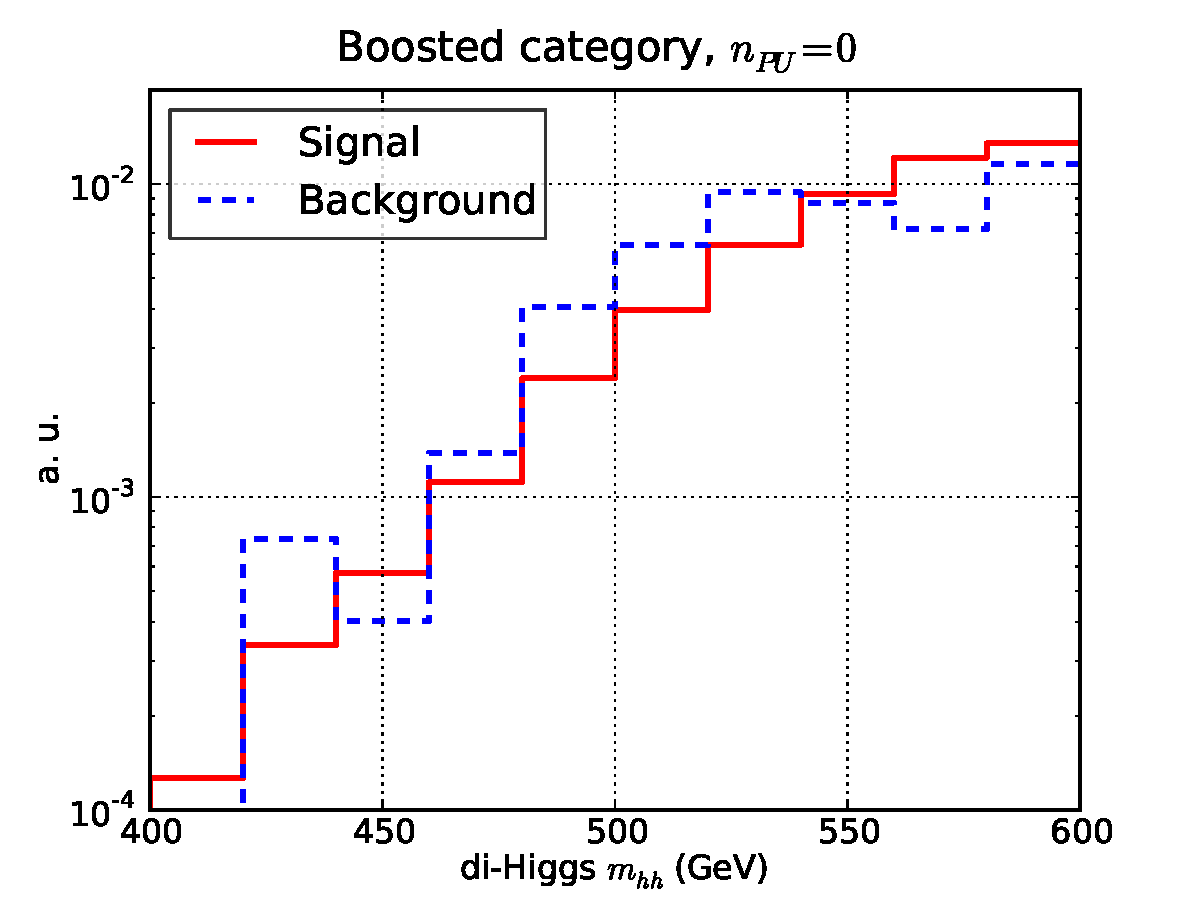
\includegraphics[width=0.48\textwidth]{plots/m_HH_C2_bst_noPU.pdf}
  \caption{\small
Same as   Fig.~\ref{fig:cutplots1} for the invariant
mass distribution of the di-Higgs system $m_{hh}$, in
the resolved (left plot) and boosted (right plot) categories.
}
\label{fig:mhh}
\end{center}
\end{figure}
%%%%%%%%%%%%%%%%%%%%%%%%%%%%%%%%%%%%%%%%%%%%%%%%%

In the resolved case, we see that the distribution
in $m_{hh}$ is rather harder for the signal as compared
to the background,
and thus one expects that cutting in $m_{hh}$ would help signal
discrimination: we will verify this using the MVA.
%
For the boosted category the overall trend of the $m_{hh}$ distribution
is different because of the jet selection cuts, with the
distribution now peaking at higher values of the invariant mass.
%
In this case, signal and background distributions
look reasonably similar.
%
Note that at parton-level the $m_{hh}$ distribution
for signal events has a kinematic
cut-off at $m_{hh}^{\rm min}=250$ GeV, which is smeared due
to 
the parton shower and to detector resolution effects.
%


In Fig.~\ref{fig:pthh} we show the transverse momentum of
the di-Higgs system, $p_T^{hh}$,
for the resolved and boosted categories.
%
Again we see that the background has a steeper $p_T^{hh}$ distribution
that the signal, in both categories, thus this variable
should provide additional discrimination power, and therefore
this distribution will be another of the inputs for the MVA.
%
In our LO simulation the $p_T^{hh}$ distribution is generated
by the parton shower, and and improved theoretical
description would require
either the matching with higher-multiplicity
matrix elements~\cite{Maierhofer:2013sha} or
the full NLO calculation~\cite{Frederix:2014hta},
%
Nevertheless, as we will show,
the MVA shows only limited sensitivity to this variable, so its
modelling is not crucial in this specific application.

%%%%%%%%%%%%%%%%%%%%%%%%%%%%
\begin{figure}[t]
\begin{center}
  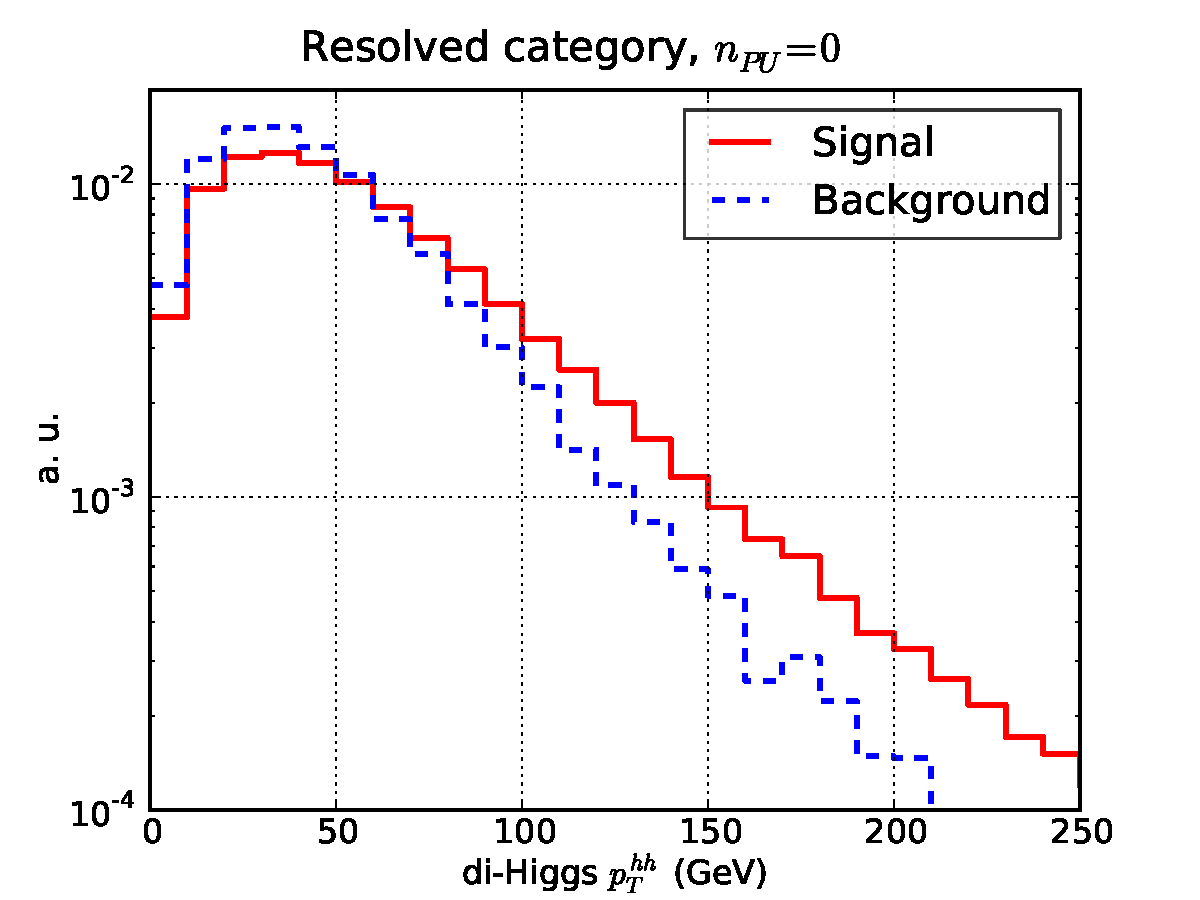
\includegraphics[width=0.48\textwidth]{plots/pt_HH_C2_res_noPU.pdf}
  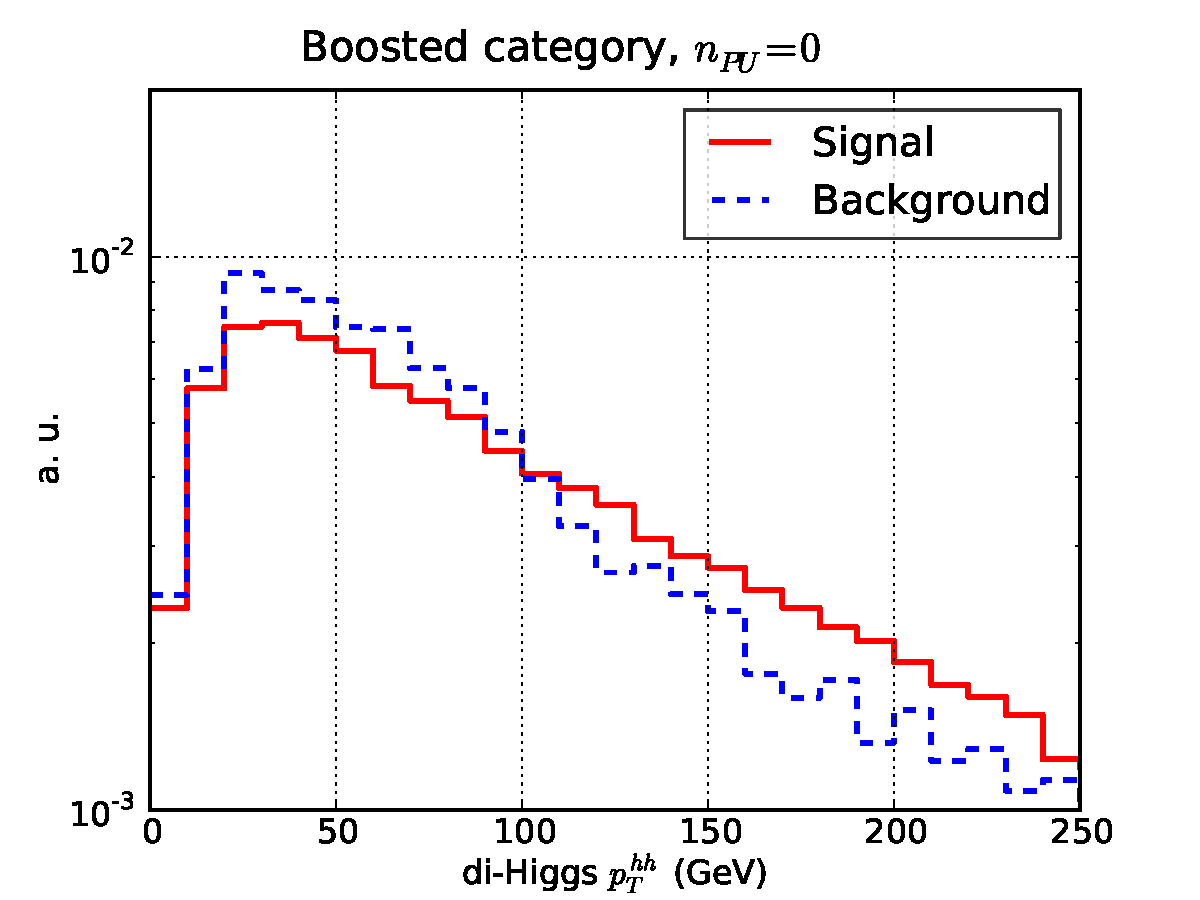
\includegraphics[width=0.48\textwidth]{plots/pt_HH_C2_bst_noPU.pdf}
  \caption{\small Same as Fig.~\ref{fig:mhh} for the transverse momentum
    distribution of the di-Higgs system $p_T^{hh}$.
}
\label{fig:pthh}
\end{center}
\end{figure}
%%%%%%%%%%%%%%%%%%%%%%%


We now study the discrimination power to separate signal
and background events contained in the jet substructure
variables.
%
In Fig.~\ref{fig:mva_substructure_1}
we show the distributions of some of
these substructure variables for the boosted category: the
$k_t$ splitting scale $\sqrt{d_{12}}$, Eq.~(\ref{eq:ktsplitting}), for
the subleading Higgs,
the energy correlation double ratio $D_2^{(\beta)}$,
Eq.~(\ref{eq:d2}), for the leading Higgs,
and then 
the 2--to--1 subjettiness ratio $\tau_{12}$,
Eq.~(\ref{eq:tau21}),
for both the leading and subleading Higgs candidates.
%

%%%%%%%%%%%%%%%%%%%%%%%%%%%%%%%%%%%%%%%%%%%%%%%%%%%%%%%
\begin{figure}[t]
  \begin{center}
    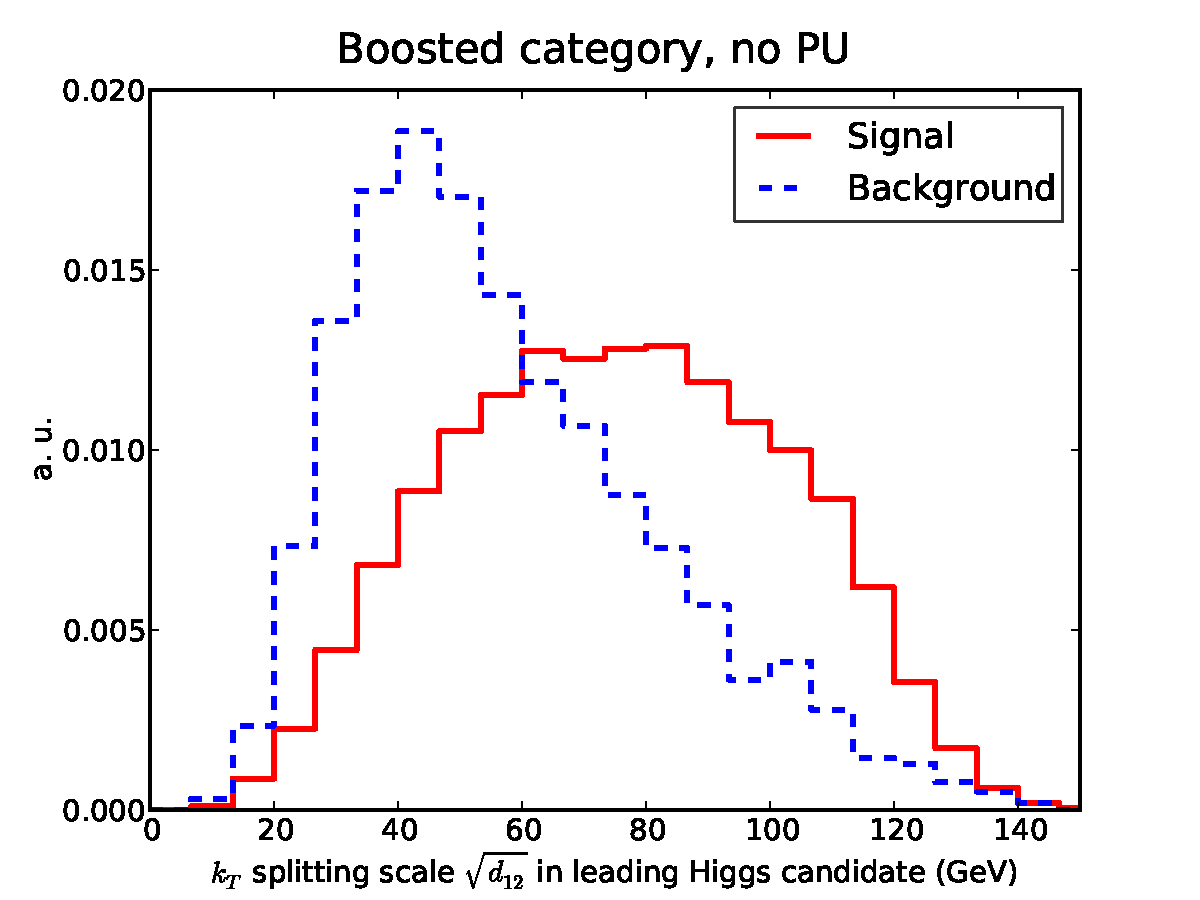
\includegraphics[width=0.48\textwidth]{plots/split12_h1_C1_boost.pdf} 
  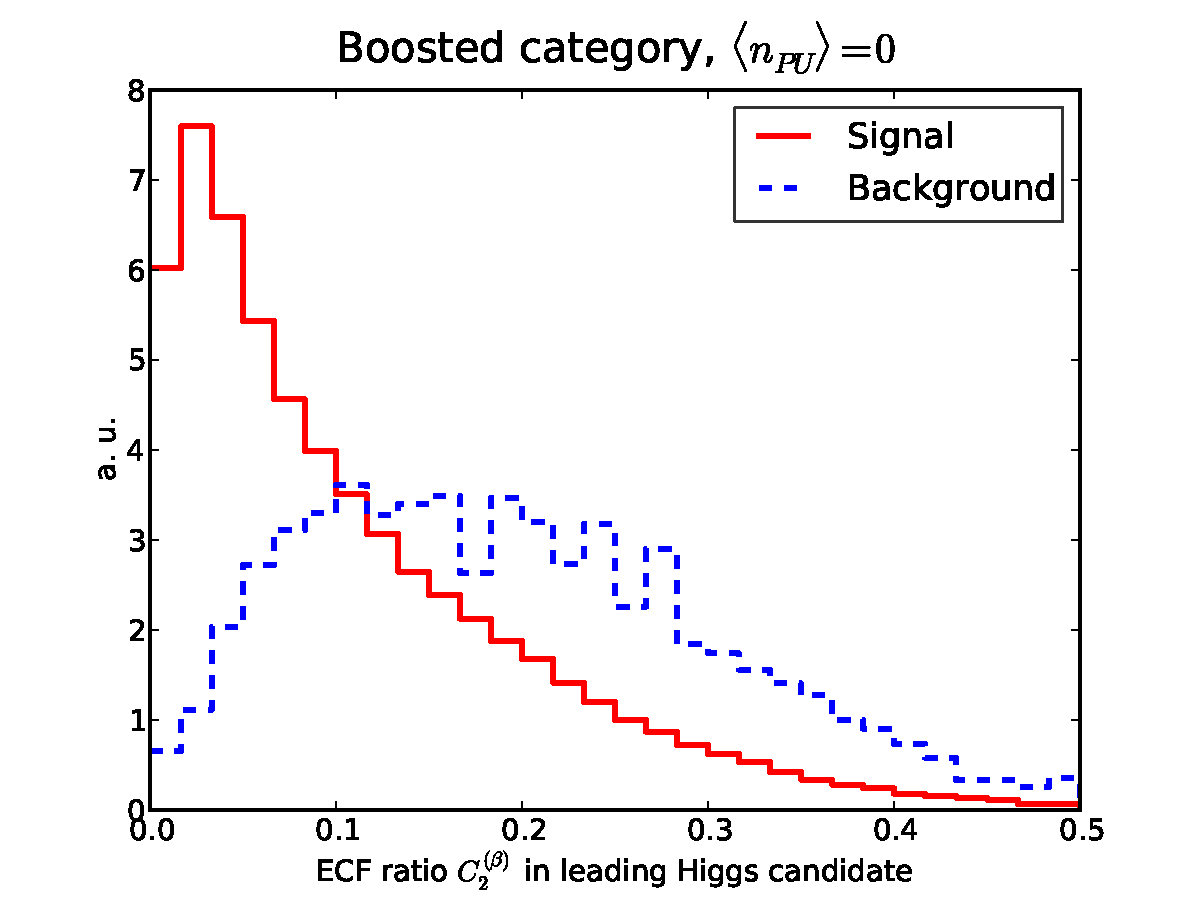
\includegraphics[width=0.48\textwidth]{plots/EEC_C2_h0_C1_boost.pdf}
  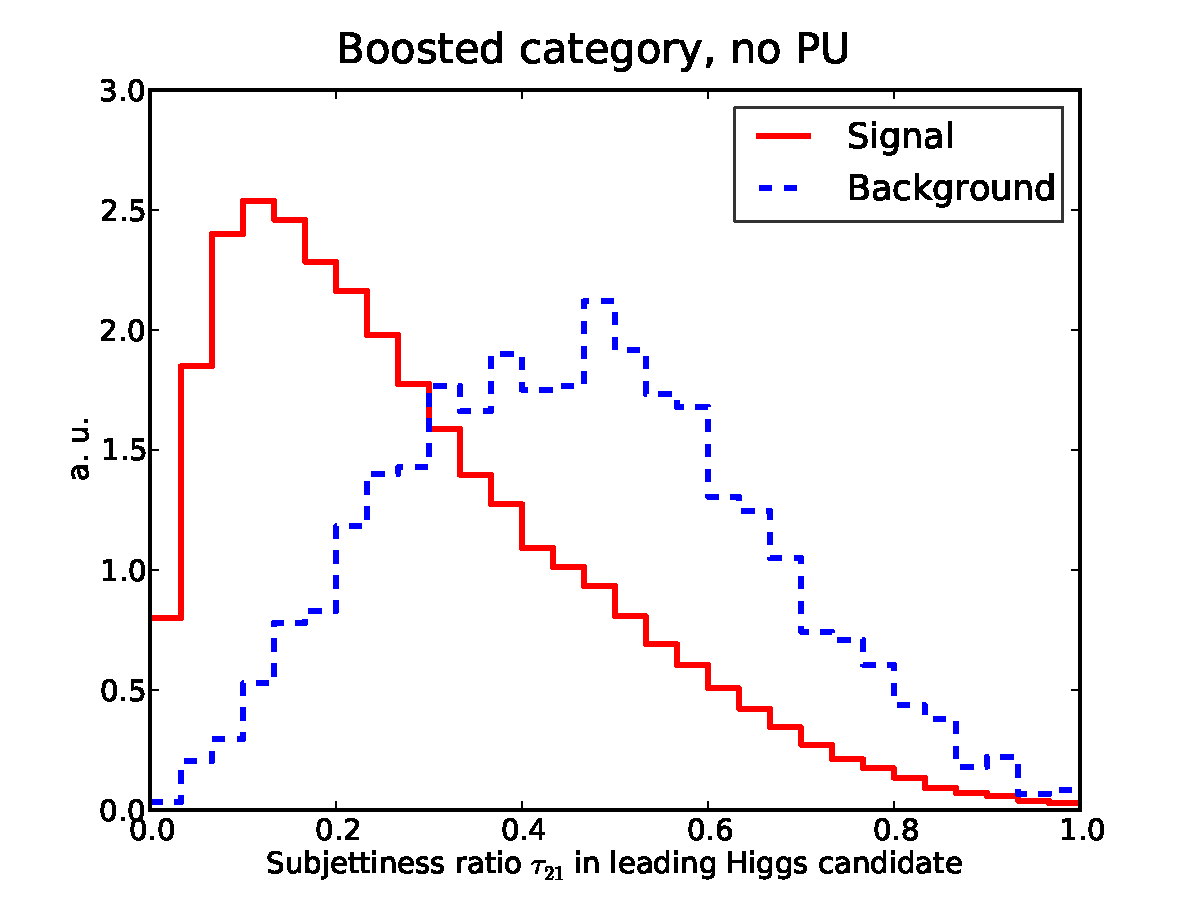
\includegraphics[width=0.48\textwidth]{plots/tau21_h0_C1_boost.pdf}
  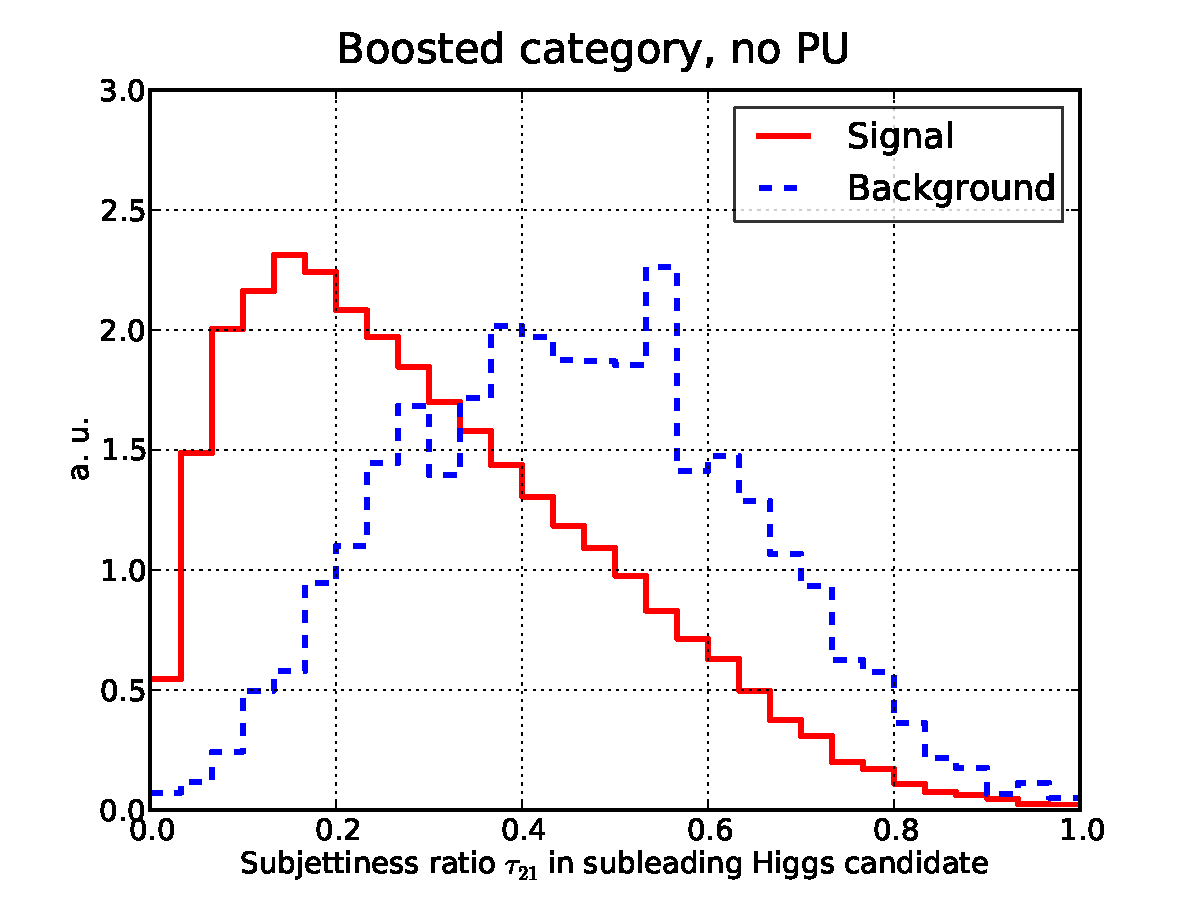
\includegraphics[width=0.48\textwidth]{plots/tau21_h1_C1_boost.pdf}
  \caption{\small Distribution of representative substructure variables
    in the boosted category at the end of the cut-based
    analysis, to be used as input to the MVA.
    %
    From top to bottom and from left to right we show  the
    $k_t$ splitting scale, the energy correlation double ratio $D_2^{(\beta)}$
    and the  subjettiness ratio $\tau_{21}$ for the leading
    Higgs, as well as $\tau_{21}$ also for the subleading Higgs.
}
\label{fig:mva_substructure_1}
\end{center}
\end{figure}
%%%%%%%%%%%%%%%%%%%%%%%%%%%%%%%%%%%%%%%%%%%%%%%%%%%%%%%%%%%%%%%%%%%


From Fig.~\ref{fig:mva_substructure_1}
we can observe that for these substructure variables the shapes of the signal
and background distributions show important differences,
reflecting the inherent differences in the internal structure of jets
between QCD jets and jets originated from the Higgs decays.
%
Importantly, we observe that signal and background distributions peak
in different regions: for example, the $k_t$ splitting scale $\sqrt{d_{12}}$
peaks around 80 GeV (50 GeV) for signal (background) events, while
the ECF ratio $D_2^{(\beta)}$ peaks at much smaller
values for signal than
for background events.
%
From Fig.~\ref{fig:mva_substructure_1} we also see
the distributions of the subjettiness ratio $\tau_{12}$ are similar
in the leading and in the subleading jets, therefore the information
contained in
$\tau_{12}$ from each of the two Higgs candidates  will be to some
extent redundant.

Therefore, while we do not explicitly have cuts in the substructure
variables, their discrimination power between signal and
background events is the motivation to include them
as input to the MVA, as we will explain in Sect.~\ref{sec:mva}.


\subsection{Impact of pile-up}
\label{sec:pileup}

Now we turn to discuss how the description of kinematic
distributions for $hh\to 4b$ signal
and background processes are
modified in a high pile-up (PU) environment.
%
To study the impact of PU,
Minimum Bias (MB) events,
including Multiple Parton Interactions (MPI), have been generated
with {\tt Pythia8}, and then
superimposed to the signal
and background samples described in Sect.~\ref{mcgeneration}.
%
We have explored two scenarios,
one with a mean number of
PU vertices per bunch crossing of $\la n_{\rm PU}\ra=80$, and another
with $\la n_{\rm PU}\ra=150$.
%
While the latter is closer to the HL-LHC forecasts,
we adopt $\la n_{\rm PU}\ra=80$ as our baseline,
given that it
is beyond the scope of this paper to fully optimize
PU subtraction,


%
In order to subtract PU in hadronic collisions, a number of techniques
are available~\cite{Cacciari:2009dp,TheATLAScollaboration:2013pia,Butterworth:2008iy,Cacciari:2007fd,Krohn:2009th,Krohn:2013lba,Ellis:2009me,Bertolini:2014bba,Cacciari:2014gra,Cacciari:2014jta,Berta:2014eza,Larkoski:2014wba}.\footnote{
These techniques have also important applications in the subtraction
of the UE/MPI contamination for jet reconstruction
in heavy ion collisions~\cite{Cacciari:2010te}.
}
%
In this work, PU  will be subtracted by means
of the {\tt SoftKiller} (SK)
method~\cite{Cacciari:2014gra}, as implemented in {\tt FastJet},
whose performance has been shown to
improve the commonly used area-based subtraction~\cite{Cacciari:2009dp}.
%
The idea underlying {\tt SoftKiller} is based on eliminating particles
below a given cut-off in their transverse momentum, $p_T^{\rm (cut)}$, whose
value is dynamically determined in a way that makes the event-wide
transverse-momentum flow density $\rho$ vanish.
%
This $p_T$ flow density is defined as
\be
\rho\equiv{\rm median}_i \Bigg\{ \frac{p_{Ti}}{A_i}\Bigg\} \, ,
\ee
where the median is computed over all the patches $i$ with area
$A_i$ and transverse momentum $p_{Ti}$ in which the $\lp \eta,\phi\rp$ plane
is partitioned.
%
From its definition in terms of the median,
it follows that the value of $p_T^{(\rm cut)}$
will be dynamically raised until half of the patches have
$p_{Ti}=0$.
%
The size and number of these patches is a free parameter of the algorithm -
here we will use square patches with length $a=0.4$.
%
We restrict ourselves to the central rapidity region,
$|\eta| \le 2.5$, for the estimation of the
$p_T$ flow density $\rho$.
%
We apply {\tt SoftKiller}
to particles at the end of the parton shower, before
jet clustering.


%%%%%%%%%%%%%%%%%%%%%%%%
\begin{figure}[t]
  \begin{center}
  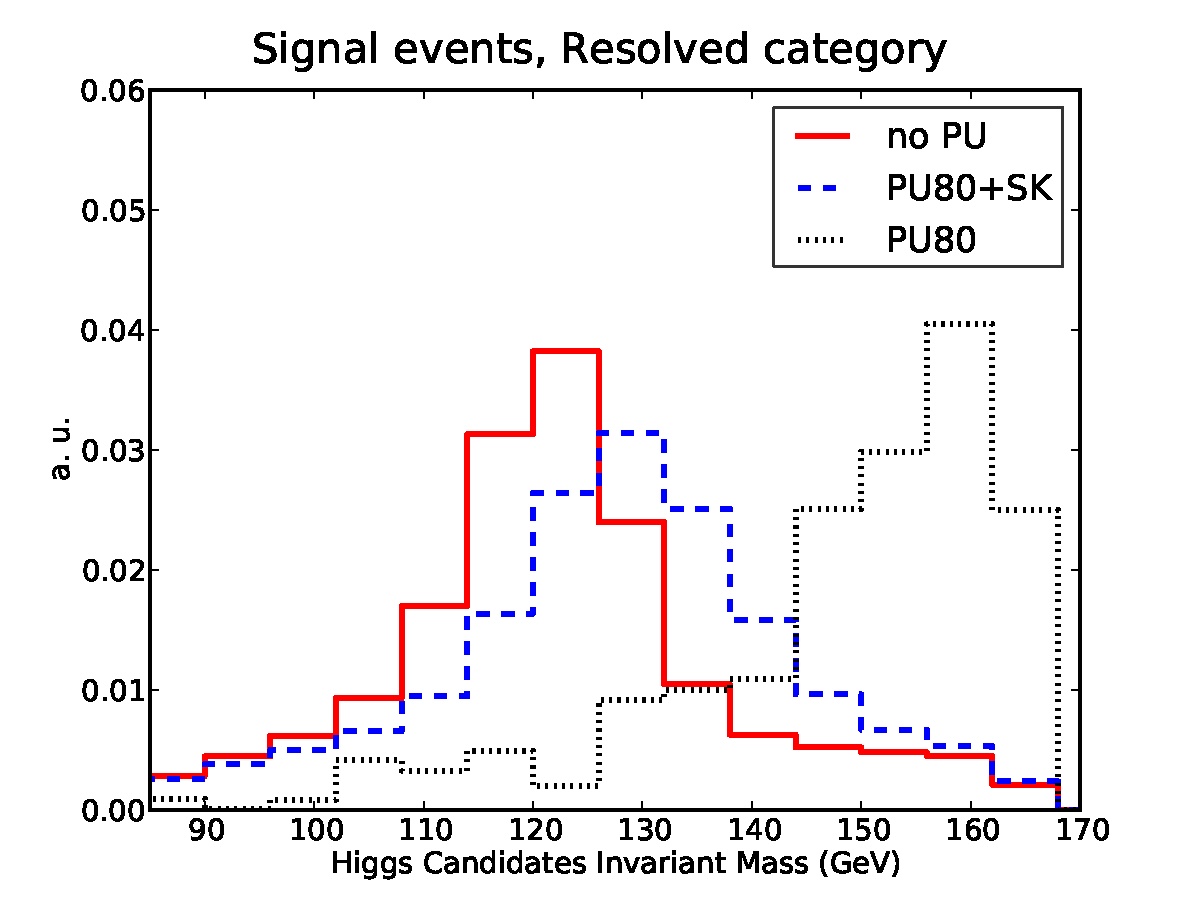
\includegraphics[width=0.63\textwidth]{plots/m_htot_res_signal_PUnoSK.pdf}
    \caption{\small
    The invariant mass distributions of Higgs candidates in signal
events, in the resolved category, comparing the results without PU,
with PU $\la n_{\rm PU}\ra=80$ but without any subtraction, and the
corresponding results now with SK subtraction.
}
\label{fig:PUvalidation}
\end{center}
\end{figure}
%%%%%%%%%%%%%%%%%%%%%%%

To validate PU subtraction,
we now compare representative kinematic distributions
in the case without PU and in the case
with PU subtracted with {\tt SoftKiller}.
%
We compare first
in Fig.~\ref{fig:PUvalidation} the
invariant mass distributions of Higgs candidates for signal
events in the resolved category.
%
We show three curves: without PU,
with PU $\la n_{\rm PU}\ra=80$ but without any subtraction, and the
same but now with the SK subtraction.
%
If PU is not subtracted there is a large shift in the Higgs mass
peak, by about 40 GeV.
%
Once SK subtraction is performed, we recover a distribution much closer
to the original ones, with only a small shift of $\simeq 5$ GeV
and a broadening of the mass
distribution.
%


Next, we compare additional
 distributions with
and without PU, with $\la n_{\rm PU}\ra=80$ in the
former
case (and SK subtraction).
%
In Fig.~\ref{fig:m_H_PU} we show the invariant mass distribution
of the leading and subleading Higgs candidates,
this time corresponding
to the boosted category.
%
These distributions are plotted after the $b$-tagging, that is,
before they are used as input to the MVA.
%
As we can see, the residual effects of PU
after the {\tt SoftKiller} subtraction are smaller
in the boosted selection as compared to the resolved case,
with the position of the Higgs mass peaks essentially
unchanged, and only a moderate broadening of the
mass distribution.
%

%%%%%%%%%%%%%%%%%%%%%%%%
\begin{figure}[t]
  \begin{center}
      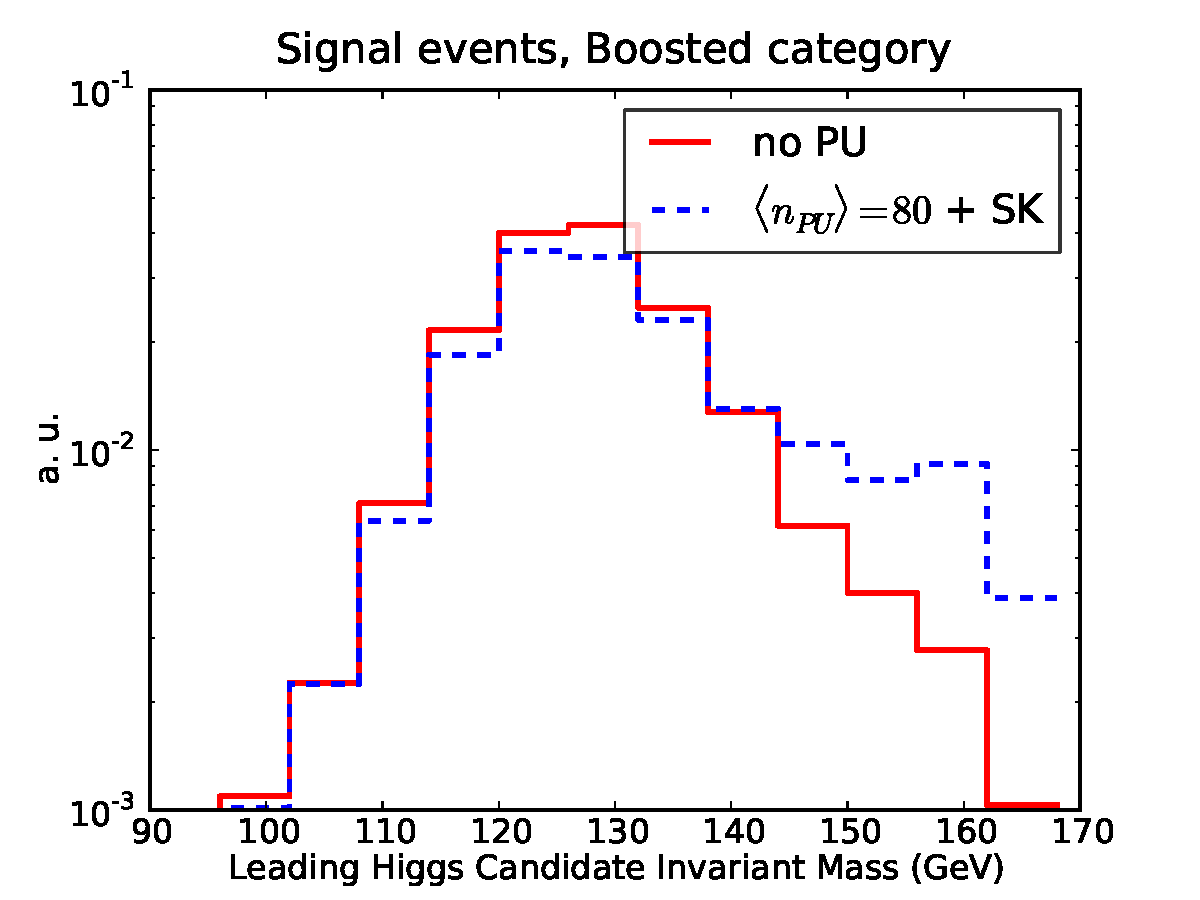
\includegraphics[width=0.49\textwidth]{plots/m_H0_bst_comp.pdf}
      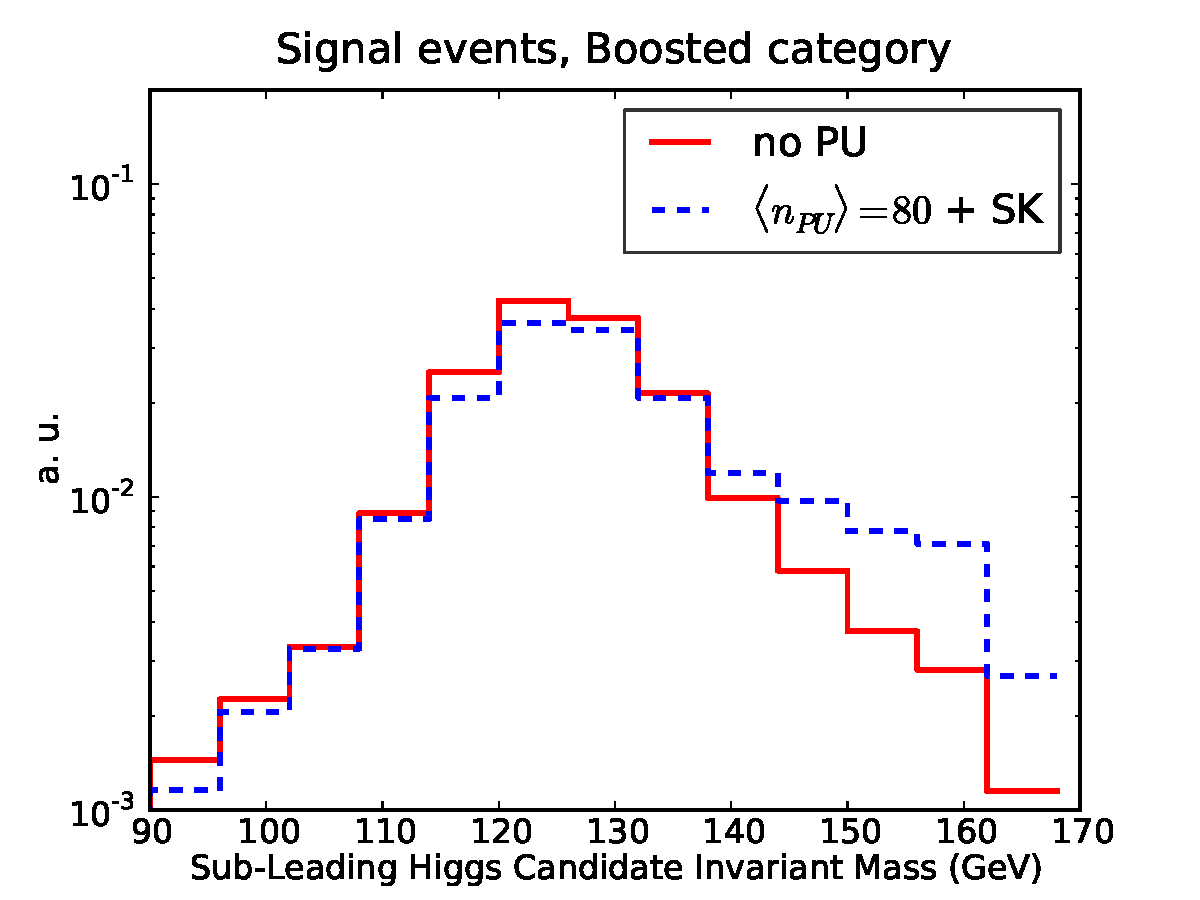
\includegraphics[width=0.49\textwidth]{plots/m_H1_bst_comp.pdf}
  \caption{\small
    Comparison of the invariant mass distributions of the leading (left plot)
    and subleading (right plot) Higgs candidates
    in the boosted category,
    both without PU and with
    PU, $\la n_{PU}\ra=80$, subtracted with {\tt SoftKiller}.
}
\label{fig:m_H_PU}
\end{center}
\end{figure}
%%%%%%%%%%%%%%%%%%%%%%%

In Fig.~\ref{fig:mHH_PU}
we compare the transverse momentum of the leading Higgs
candidate, $p_t^{h_1}$ and the invariant mass of the di-Higgs system
$m_{hh}$, in both for the boosted and
for the resolved categories.
%
In the case of the $p_T^{h1}$ distribution, the differences between the selection
criteria for the resolved
and boosted categories is reflected in the rightward shift of the latter.
%
The effect of PU is small in the boosted case, and generally moderate
in the resolved case, except for large $p_T$ values.
%
Similar observation can be derived for the case of
the di-Higgs invariant mass $m_{hh}$ distribution, similar 
apply.
%
Therefore, we can consider the PU subtraction strategy
as validated for the purposes of this study, although
there could still be room for optimisation.


%%%%%%%%%%%%%%%%%%%%%%%%
\begin{figure}[t]
  \begin{center}
  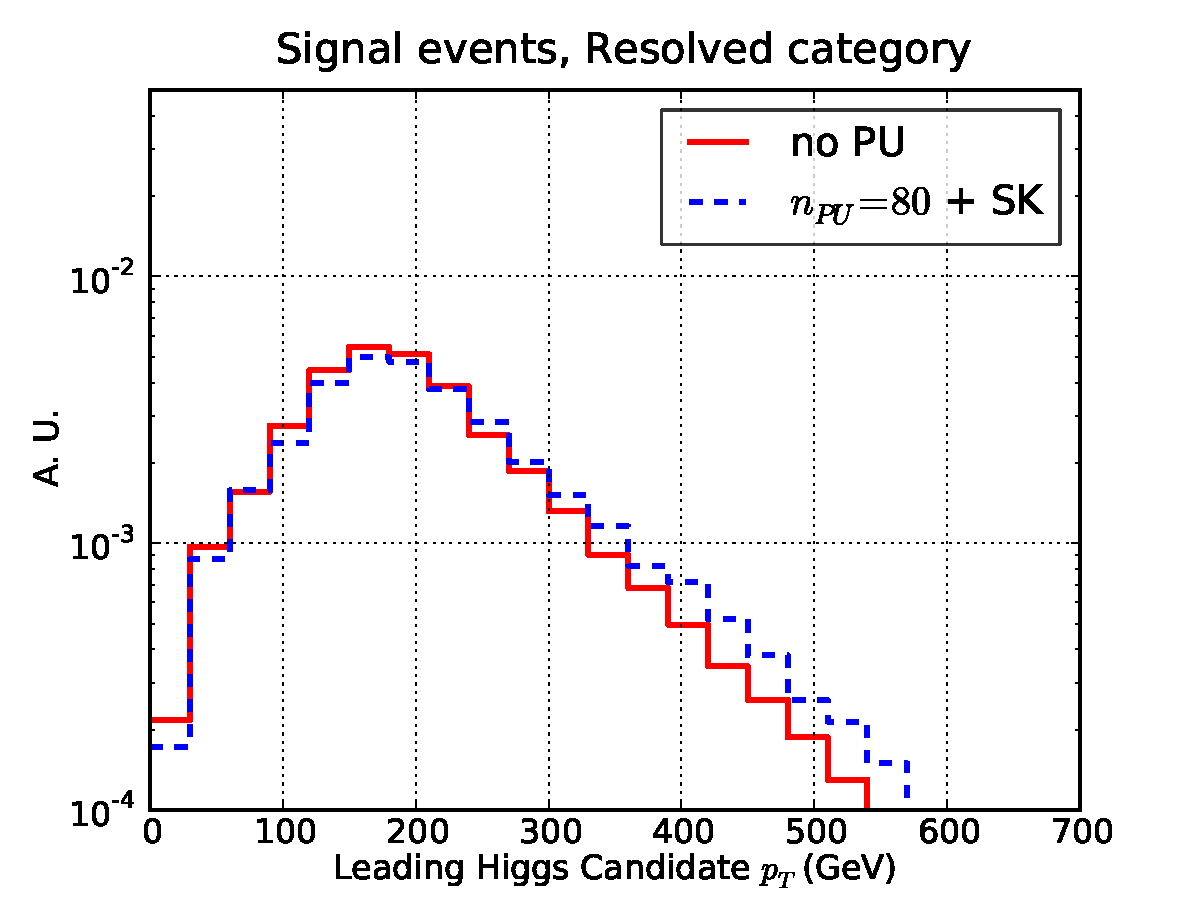
\includegraphics[width=0.49\textwidth]{plots/pt_H0_C2_res_comp.pdf}
  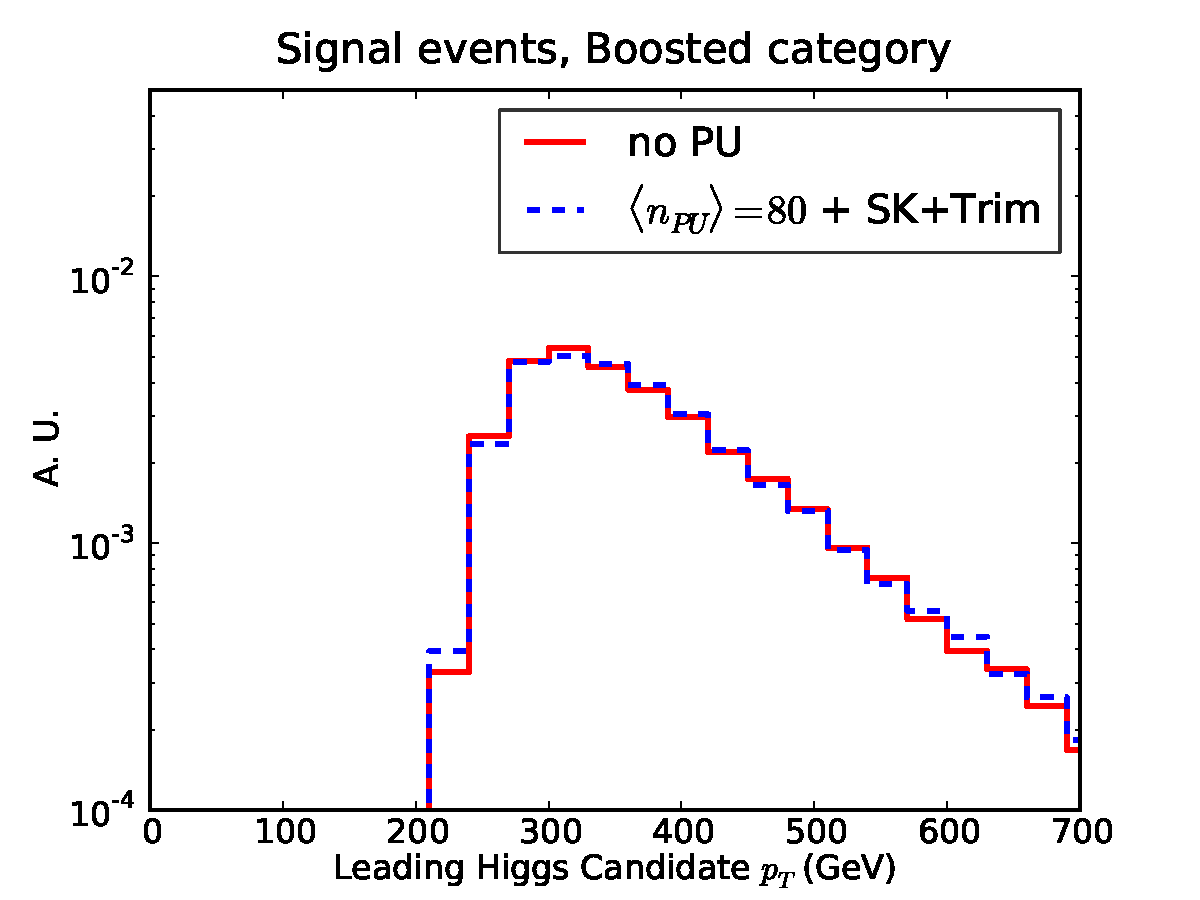
\includegraphics[width=0.49\textwidth]{plots/pt_H0_C2_bst_comp.pdf}
  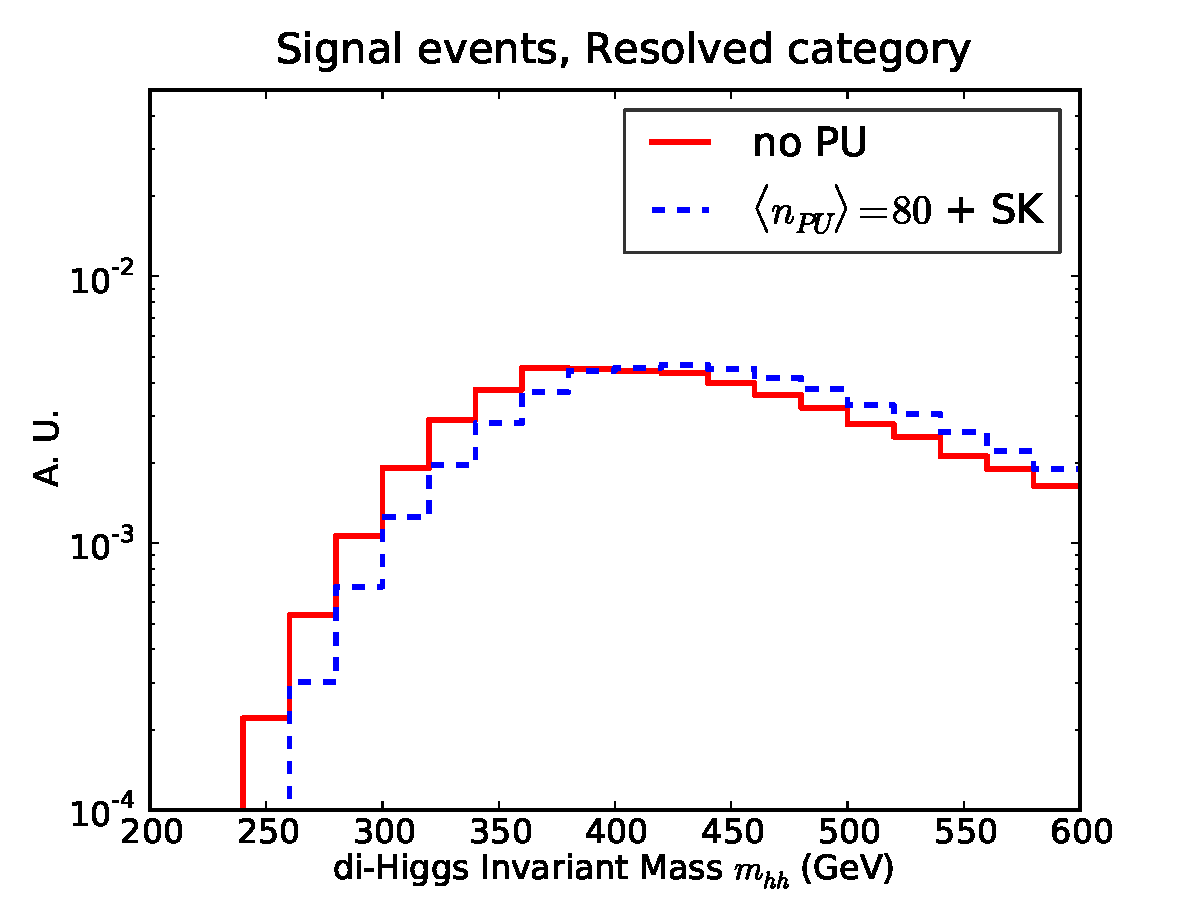
\includegraphics[width=0.49\textwidth]{plots/m_HH_C2_res_comp.pdf}
  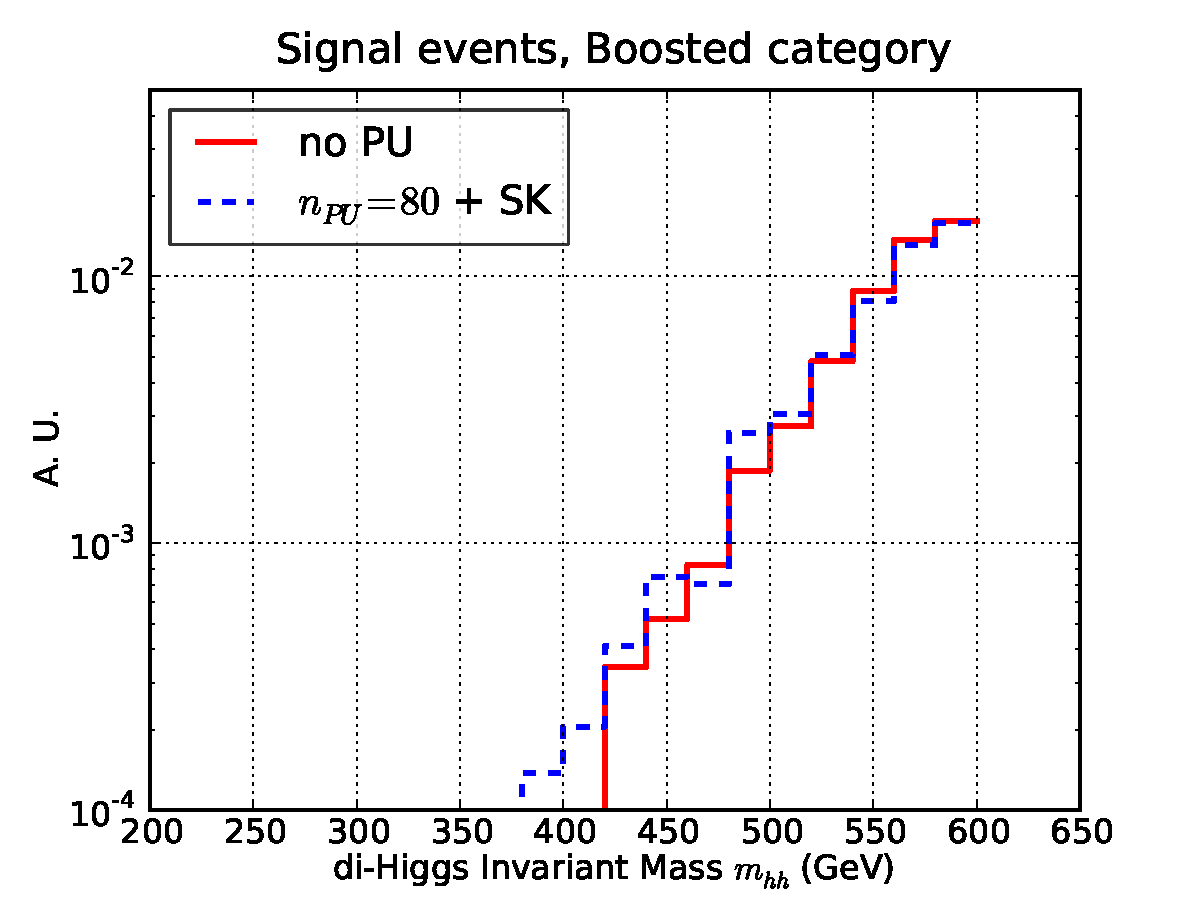
\includegraphics[width=0.49\textwidth]{plots/m_HH_C2_bst_comp.pdf}
  \caption{\small
    Comparison of the transverse momentum $p_T^h$ of the leading
    Higgs candidate (upper plots) and of the invariant mass $m_{hh}$
    of the di-Higgs system (lower plots) in the resolved
    (left plots) and boosted (right plots) categories,
    without PU and with $\la n_{PU}\ra=80$ subtracted with {\tt SoftKiller}.
}
\label{fig:mHH_PU}
\end{center}
\end{figure}
%%%%%%%%%%%%%%%%%%%%%%%

We can also assess the impact of PU in some of
substructure variables that will be 
used as input to the MVA in the boosted category.
%
In Fig.~\ref{fig:Substructure_PU} we show the 2-to-1 subjettiness ratio
$\tau_{21}$, Eq.~(\ref{eq:tau21}), and the ratio
of energy correlation functions, $D_2^{(\beta)}$,
Eq.~(\ref{eq:d2}), in both cases
corresponding to the leading Higgs candidate.
%
Comparing the signal distributions in the cases without PU and
with PU subtracted with SK, we observe that both substructure variables
are reasonably robust in a high-PU environment.
%
The ratio of energy correlation functions $D_2^{(\beta)}$ 
was indeed constructed~\cite{Larkoski:2013eya}
to be resilient
with respect to PU contamination.
%

%%%%%%%%%%%%%%%%%%%%%%%%
\begin{figure}[t]
  \begin{center}
  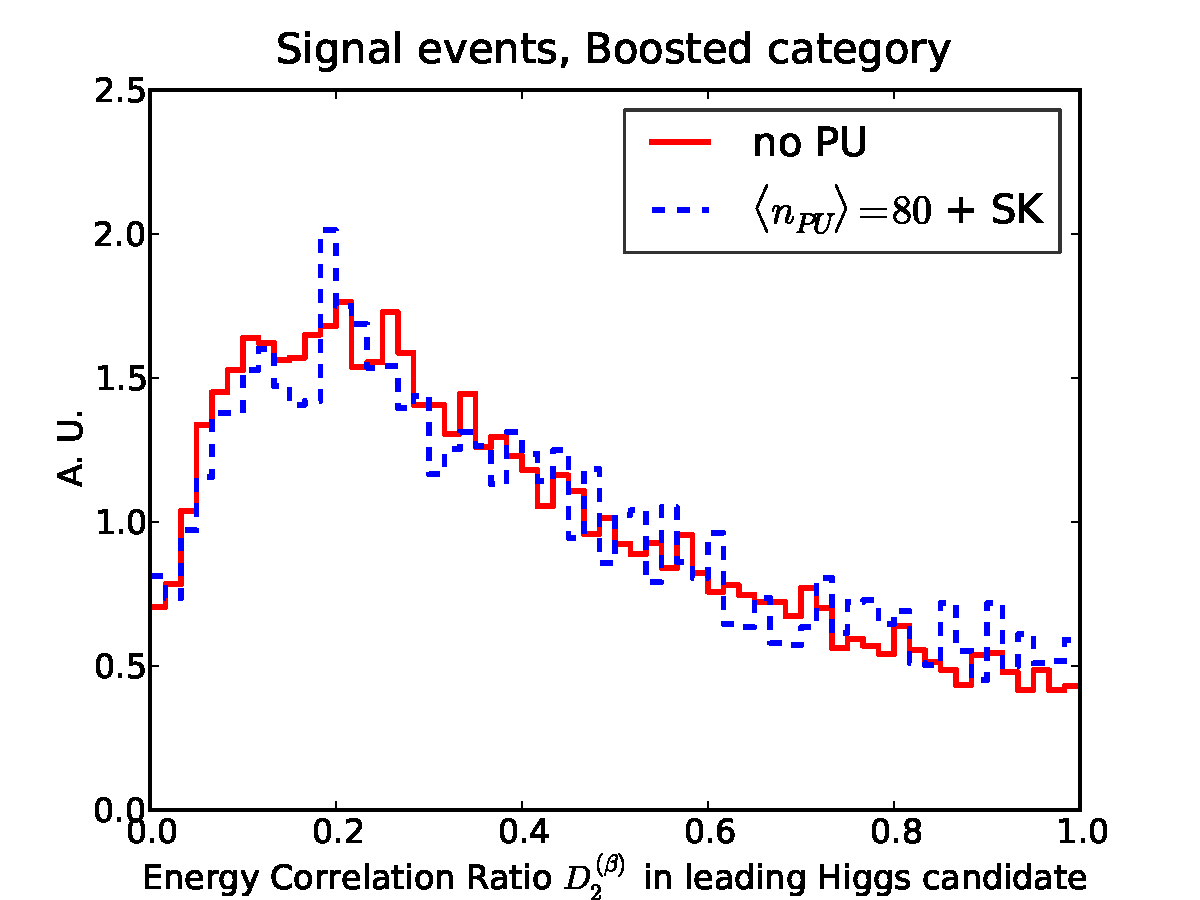
\includegraphics[width=0.49\textwidth]{plots/D2_h0_bst_comp.pdf}
  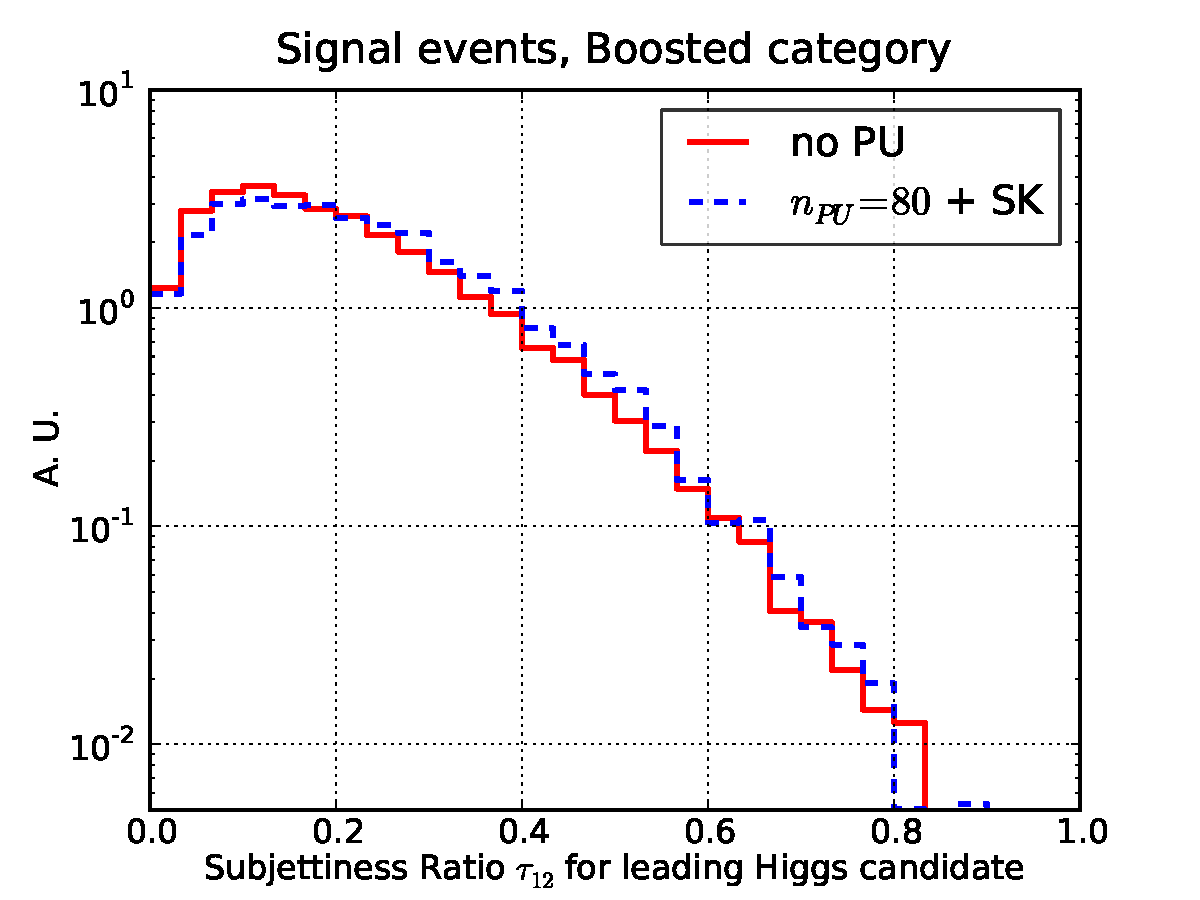
\includegraphics[width=0.49\textwidth]{plots/tau21_h0_bst_comp.pdf}
   \caption{\small
     Comparison of the substructure variables $D_2^{(\beta)}$ (left)
     and $\tau_{21}$ (right)
     for the leading Higgs candidate in the boosted category,
   without PU and with $\la n_{\rm PU}\ra=80$ subtracted with {\tt SoftKiller}.
}
\label{fig:Substructure_PU}
\end{center}
\end{figure}
%%%%%%%%%%%%%%%%%%%%%%%

It is also interesting to quantify how
the relative differences between
signal over background distributions are modified in a high-PU
environment.
%
Considering first of all the boosted category,
in Fig.~\ref{fig:signal-vs-back-boosted} we compare
various kinematic distributions for signal and background events,
with and without PU for the leading Higgs candidate: the invariant mass, the transverse
momentum distribution $p_T$,
     the 2--to--1 subjettiness ratio $\tau_{21}$, and 
     the $k_T$ splitting scale $\sqrt{d_{12}}$, Eq.~(\ref{eq:ktsplitting}).
     %
      We verify that the relevant
      qualitative differences between signal
      and background distributions are maintained even in the presence of PU.
      %
      This is specially noticeable for the substructure variables, which
      exhibit a similar discrimination power both with and without
      PU.
     

%%%%%%%%%%%%%%%%%%%%%%%%
\begin{figure}[t]
  \begin{center}
  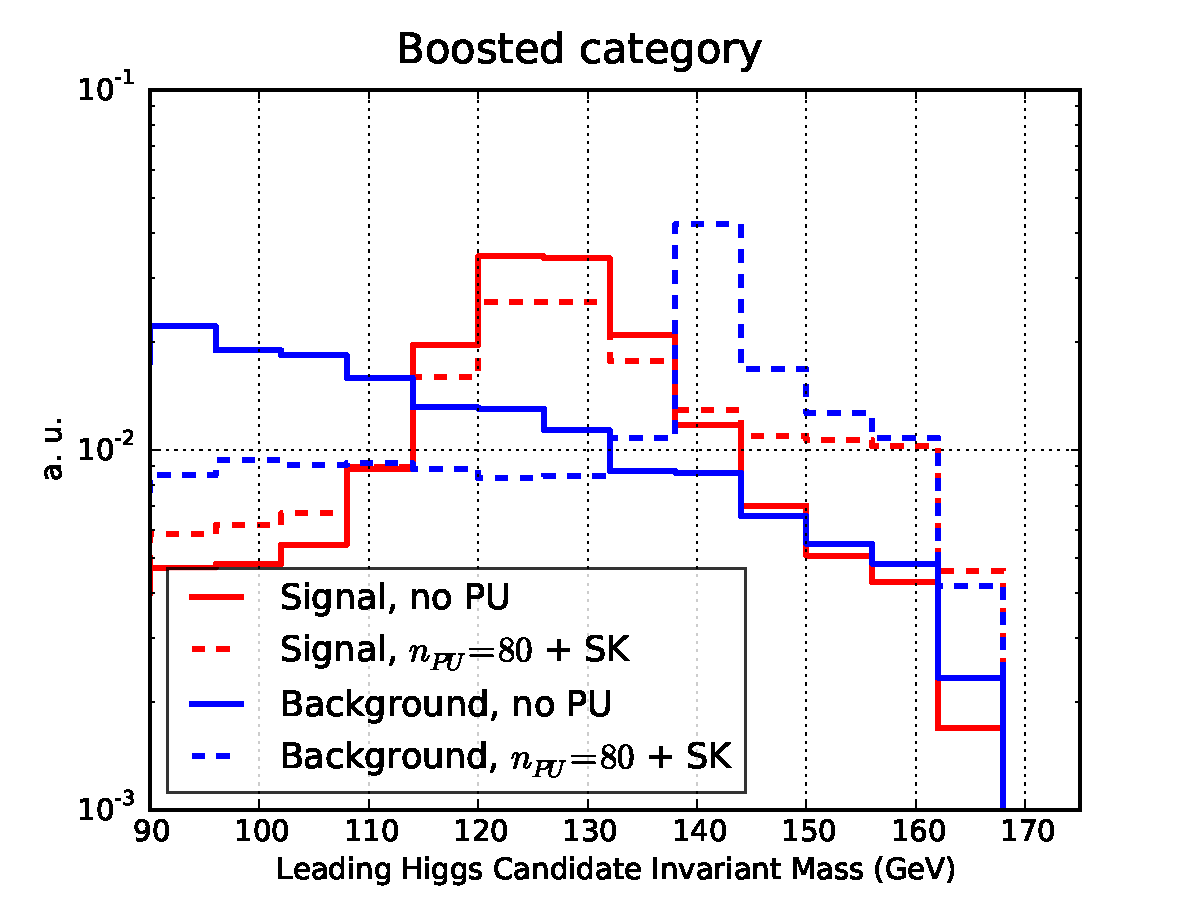
\includegraphics[width=0.49\textwidth]{plots/m_h0_bst_comp_back.pdf}
  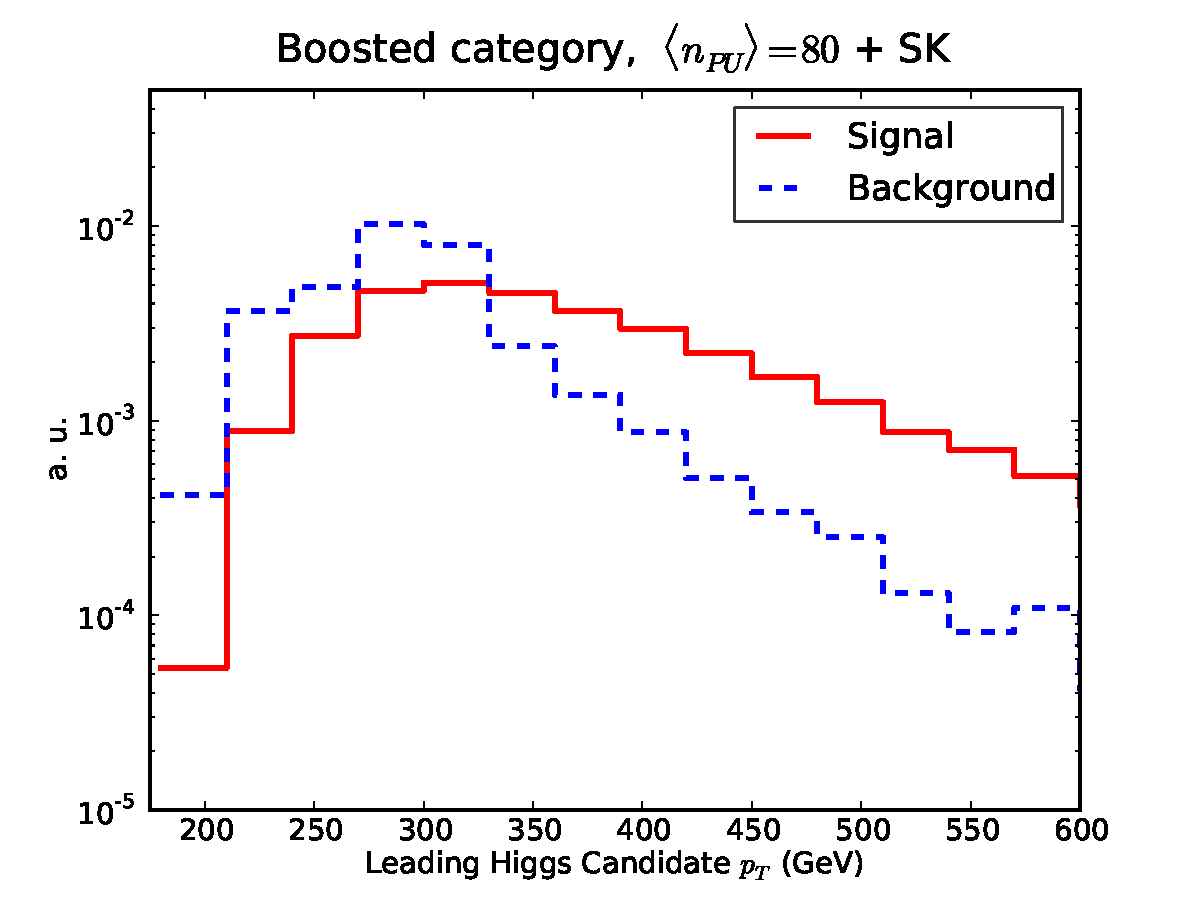
\includegraphics[width=0.49\textwidth]{plots/pt_h0_bst_comp_back.pdf}
   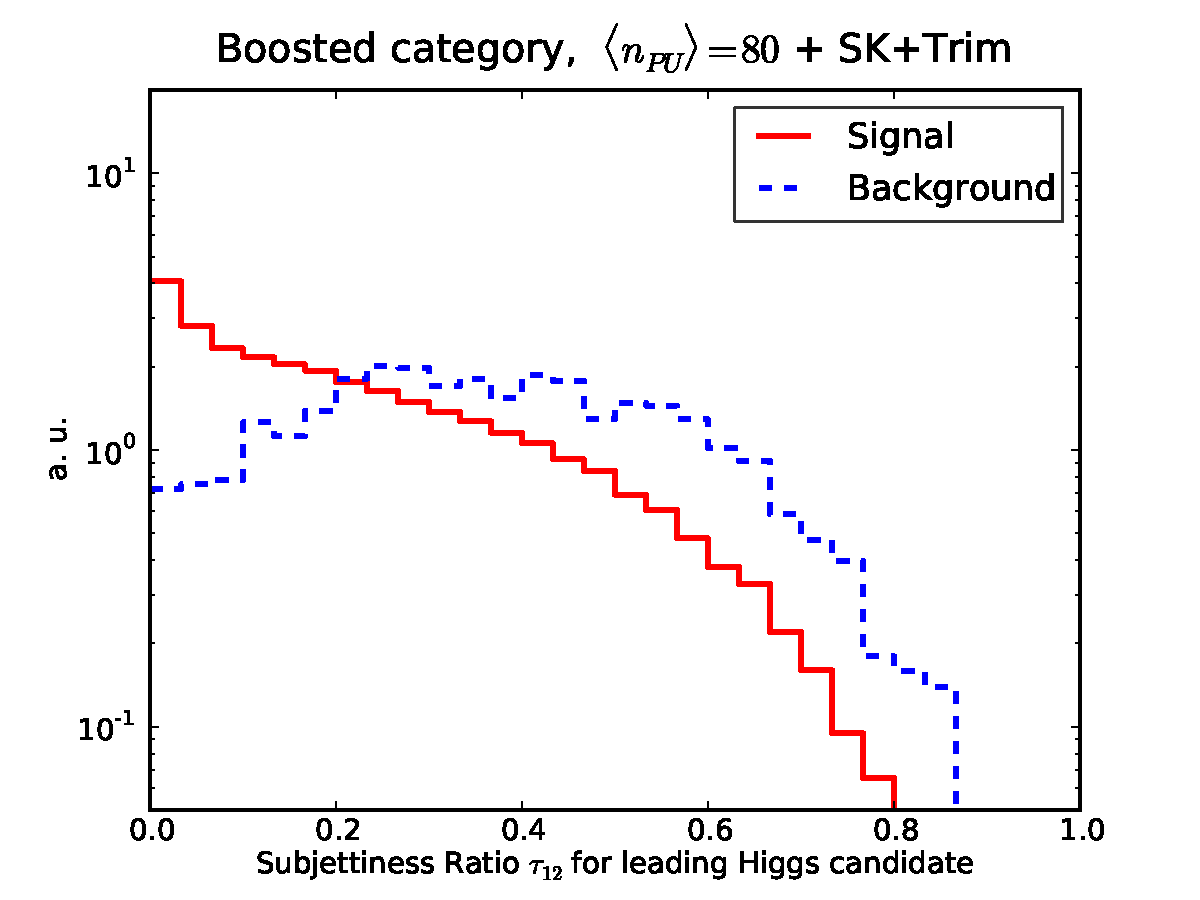
\includegraphics[width=0.49\textwidth]{plots/tau21_h1_bst_comp_back.pdf}
  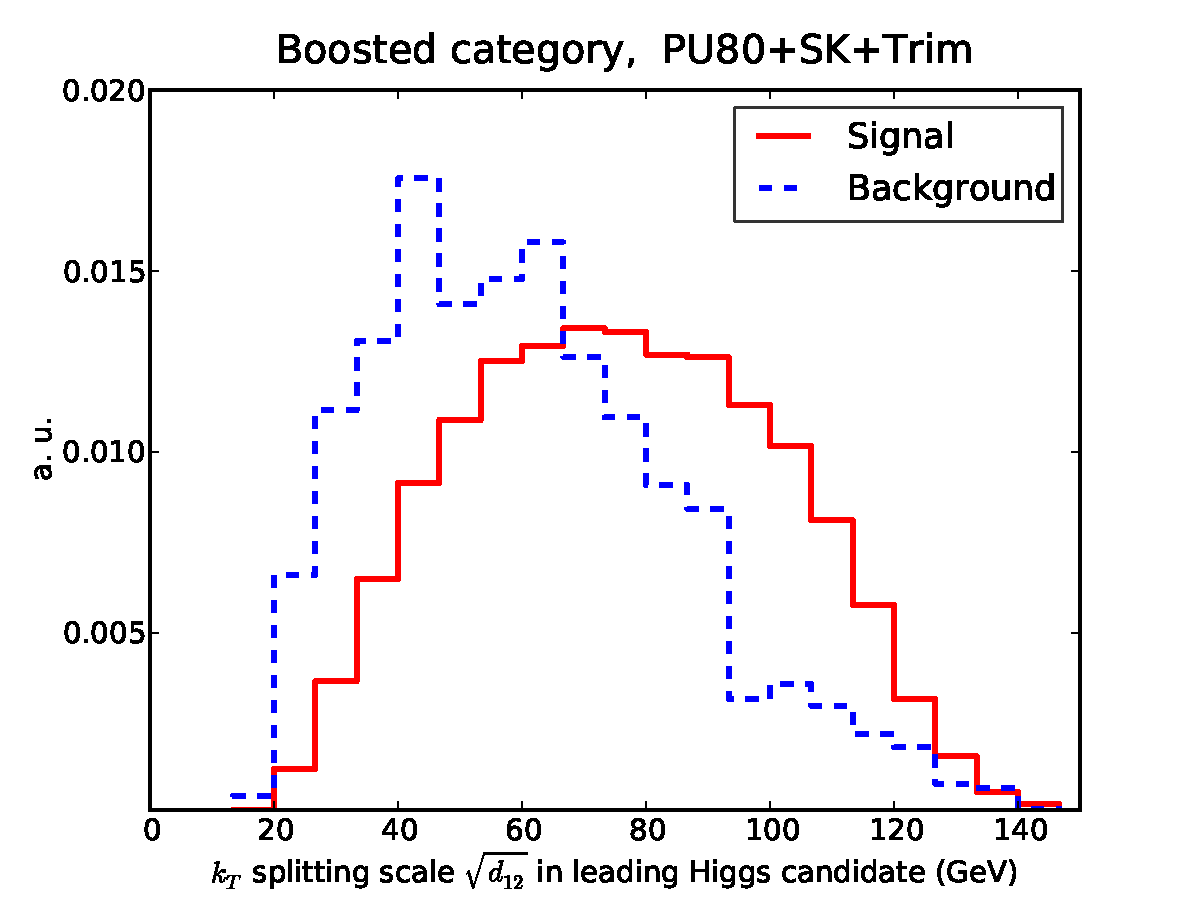
\includegraphics[width=0.49\textwidth]{plots/split12_h0_bst_comp_back.pdf}
   \caption{\small
     Comparison of kinematic distributions, in
     the boosted category, for signal and background events
     with and without PU: the invariant mass,  $p_T$,
     and the substructure variables $\tau_{21}$ and $\sqrt{d_{12}}$
    for the leading Higgs candidate.
     %
 }
\label{fig:signal-vs-back-boosted}
\end{center}
\end{figure}
%%%%%%%%%%%%%%%%%%%%%%%



Finally, can perform a similar comparison for
the resolved category.
%
In Fig.~\ref{fig:signal-vs-back-resolved} we compare
the kinematic distributions for signal and background events,
     with and without PU, for the invariant mass and the $p_T$ of the leading
     Higgs candidate.
     %
     Also in this
     case the PU-subtracted background distributions appear reasonably close
     to their no PU counterparts.

%%%%%%%%%%%%%%%%%%%%%%%%
\begin{figure}[t]
  \begin{center}
   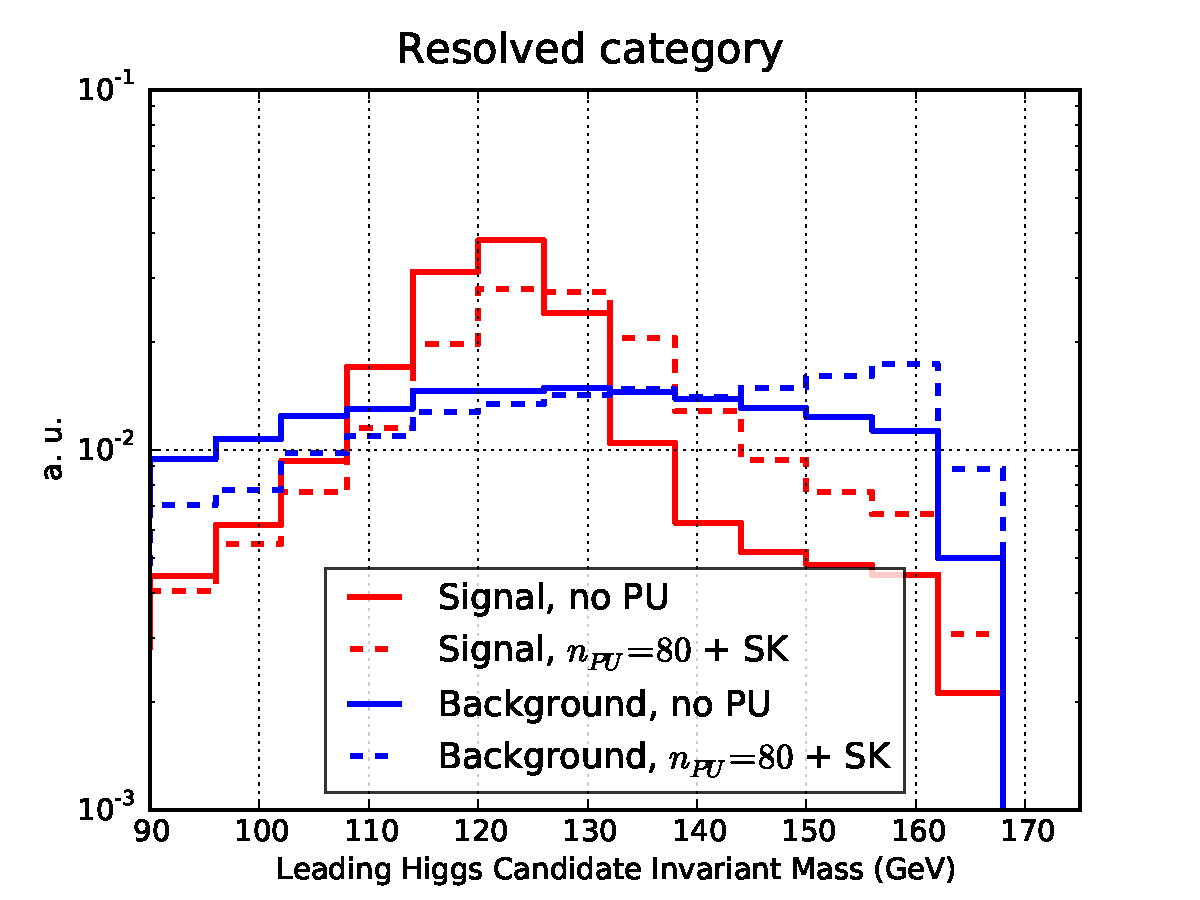
\includegraphics[width=0.49\textwidth]{plots/m_h0_res_comp_back.pdf}
  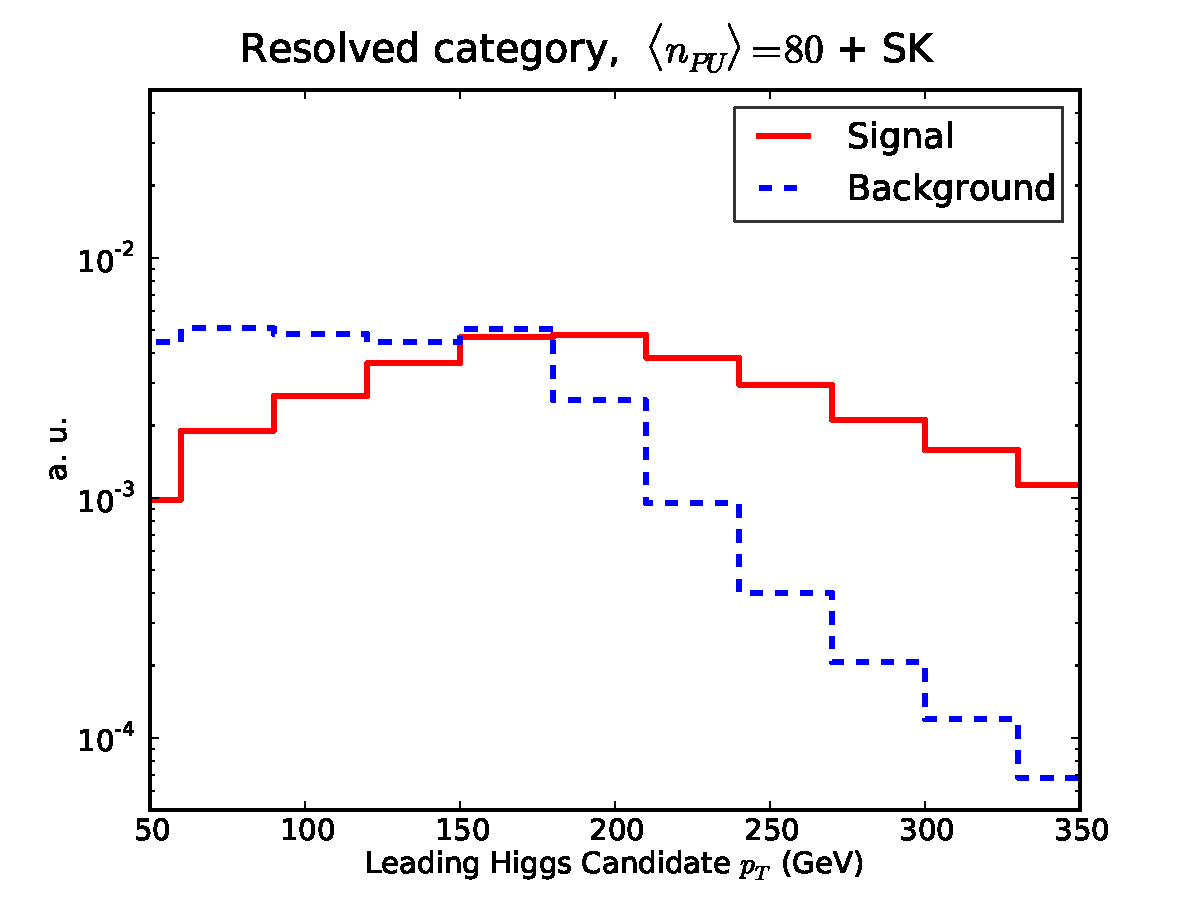
\includegraphics[width=0.49\textwidth]{plots/pt_h0_res_comp_back.pdf}
     \caption{\small
       Same as Fig.~\ref{fig:signal-vs-back-boosted} for the resolved category,
       this time without the jet substructure variables.
}
\label{fig:signal-vs-back-resolved}
\end{center}
\end{figure}
%%%%%%%%%%%%%%%%%%%%%%%



%%%%%%%%%%%%%%%%%%%%%%%%%%%%%%%%%%%%%%%%%%%%%%%%%%%
%%%%%%%%%%%%%%%%%%%%%%%%%%%%%%%%%%%%%%%%%%%%%%%%%%%
%%%%%%%%%%%%%%%%%%%%%%%%%%%%%%%%%%%%%%%%%%%%%%%%%%%
%%%%%%%%%%%%%%%%%%%%%%%%%%%%%%%%%%%%%%%%%%%%%%%%%%%
